%%%%%%%%%%%%%%%%%%%%%%%%%%%%%%%%%%%%%%%%%
% MODELE DE MANUSCRIT DE THESE 
% DE L'UNIVERSITE PARIS CITE
% OFFICIEL

% LaTeX Template
% Version overleaf (14/10/2023) 
% Format BOOK
% Par Aleksandra SAVINA, PhD
% https://www.overleaf.com/latex/templates/phd-thesis-template-universite-paris-cite/jycfrbbjbgrm
%%%%%%%%%%%%%%%%%%%%%%%%%%%%%%%%%%%%%%%%%


%----------------------------------------------------------------------------------------
%	PREAMBULE // PACKAGES AND OTHER DOCUMENT CONFIGURATIONS
%----------------------------------------------------------------------------------------
\documentclass[a4paper,12pt,twoside,french]{book}
\usepackage{PackagesDeAmbroise}
\selectlanguage{french}%
\linespread{1.2} % Line spacing of 1.5 times the normal spacing
\title{Memoire M2 ISF _ DSS_SD3_3C}
\author{Ambroise Warnery}
\date{August 2024}

% Headers footers and glossaires
\fancyhead{} % clear all header fields
\fancyfoot{} % clear all footer fields
\makeglossaries
\makeindex

%%%%%%%%%%%%%%%%%%%%%%%%%%%%%%%%%%%%%%%%%%%%%%%%%%%%%%%%%%%%%%%%%%%%%%%%%%
%%%%%%%%%%%%%%%%%%%%%%%%%%%%%%%%%%%%%%%%%%%%%%%%%%%%%%%%%%%%%%%%%%%%%%%%%%
%----------------------------------------------------------------------------------------
%	DOCUMENT
%----------------------------------------------------------------------------------------
\begin{document}

%\maketitle
%----------------------------------------------------------------------------------------
%	TITLE PAGE
%----------------------------------------------------------------------------------------
	\begin{titlepage}
		\begin{center}
				\includegraphics[height=2.5cm]{figures/cover/logoAssas.png}
		\end{center}
	
		\begin{center}
		
\vspace*{.03\textheight}
\textsc{\LARGE Université Paris-Panthéon-Assas}\\[0.2cm] % Univ name
		\large M2 - Ingénierie Statistique et Financière\\
  			\vfill
 
	 		\rule{\textwidth}{0.8pt} \\ % Horizontal line
	 		\vspace{10pt}
	 		 { \LARGE \bfseries Conception et évaluation de politiques publiques dans le cadre des retraites} % Thesis title
	 		 \vspace{10pt}
	 		 \rule{\textwidth}{0.8pt} \\ % Horizontal line
		\end{center}
		
		\vfill
		% Author and supervisor	
		\begin{center}
			Par \textsc{\Large Ambroise WARNERY}\\[1cm] 
			Mémoire d'alternance\\[1.2cm]
			Dirigée par \textsc{\large Joseph LANFRANCHI}\\[0.2cm]
            Et par \textsc{\large Taha BENABDELAZIZ}\\[0.2cm] 
			Présenté et soutenue le 27/09/2024 %renseigner la date et choisir le type de soutenance
		\end{center}
		
		\vspace{1cm}


	\newpage %page de garde vide
	\thispagestyle{empty} %page de garde vide
	\end{titlepage}

\renewcommand{\chaptermark}[1]{\markboth{#1}{}}

\frontmatter % numérote les pages en chiffres romains jusqu'a la commande mainmatter

%----------------------------------------------------------------------------------------
%	RESUME ET ABSTRACT PAGE
%----------------------------------------------------------------------------------------
\chapter*{Résumé}
\addcontentsline{toc}{chapter}{Résumé} 

\begin{mdframed}
\vspace{-.25cm}
\paragraph*{Titre:} Conception et évaluation de politiques publiques dans le cadre des retraites.

\begin{small}
\vspace{-.25cm}
\paragraph*{Mots clefs:} Réformes des retraites ; Portabilité des droits ; Travailleurs indépendants ; RATP ; Assiette sociale ; Cotisations sociales

\vspace{-.5cm}
\setlength{\columnsep}{12pt} % I want the columnsep to be wider only on this page.
\begin{multicols}{2}
\paragraph*{Résumé:} 
Ce mémoire traite de deux grandes réformes liées aux politiques publiques dans le cadre des retraites en France : l'ouverture à la concurrence des lignes de bus RATP et la réforme de l’assiette sociale des travailleurs indépendants (TI) et des professions libérales (PL). La première réforme, initiée par le droit européen, vise à garantir la portabilité des droits à la retraite des salariés transférés à de nouveaux employeurs via un "sac à dos social". Ce dispositif assure la continuité des droits sociaux des agents RATP lors de la transition vers des entreprises privées.

La seconde réforme concerne la simplification du calcul des cotisations sociales des TI et PL, en fusionnant les assiettes de cotisations et de contributions sociales (CSG et CRDS). Cela vise à réduire les inégalités entre ces professions et les salariés, tout en améliorant la transparence du système et l’acquisition de droits sociaux.

Ces deux réformes, bien que distinctes, illustrent les défis actuels d'équité, de simplification administrative et de durabilité des régimes de retraite en France, enjeux majeurs pour les politiques publiques.

\end{multicols}
\end{small}
\end{mdframed}

\clearpage
 %résumé en francais

%----------------------------------------------------------------------------------------
%	ACKNOWLEDGEMENTS
%----------------------------------------------------------------------------------------
\chapter*{Remerciements}
\addcontentsline{toc}{chapter}{Remerciements} 

Je tiens en premier lieu à remercier Taha Benabdelaziz qui a été mon tuteur d'alternance durant cette année très enrichissante. Il a su m'accompagner tout au long de l'année dans les différentes missions que nous avons eu à réaliser et m'a particulièrement aidé dans l'écriture de ce mémoire. 

\bigskip

Je souhaite également remercier Delphine Chaumel, sous directrice de la 3ème sous direction de la direction de la Sécurité Sociale, ainsi que son adjoint Hédi Brahimi, de m’avoir accueilli au sein de leur sous direction et de m’avoir permis de mener à terme ce mémoire dans les meilleures conditions.

\bigskip

Je tiens par ailleurs à remercier, l’ensemble des agents du bureau 3C et des bureaux 3A et 3B pour l'accueil qu'elles et ils m'ont fait, les discussions partagées et leurs encouragements, notamment durant les dernières semaines de rédaction de ce mémoire.

\bigskip

Sur le plan académique, je souhaite remercier également Monsieur Joseph Lanfranchi, pour ses différents conseils et sa disponibilité, ainsi que l’ensemble des professeurs du Master EFIQUAS de m’avoir fait bénéficier d’une formation de qualité.

\mbox{}
\newpage

%----------------------------------------------------------------------------------------
%	LIST OF CONTENTS/FIGURES/TABLES PAGES
%----------------------------------------------------------------------------------------
%\setcounter{secnumdepth}{3} % organisational level that receives a numbers
%\setcounter{tocdepth}{3}
\tableofcontents % Prints the main table of contents

%\listoffigures % Prints the list of figures
%\addcontentsline{toc}{chapter}{Liste des figures}

%\listoftables % Prints the list of tables
%\addcontentsline{toc}{chapter}{Liste des tableaux}

\newpage

%----------------------------------------------------------------------------------------
%	Liste des abréviations-
%----------------------------------------------------------------------------------------
%\chapter*{Liste des abréviations}
%\addcontentsline{toc}{chapter}{Liste des abréviations} 

\printacronyms[type=\acronymtype, title=Liste des abréviations, toctitle=Liste des abréviations]

\newacronym{RATP}{RATP}{Régie Autonome des Transports Parisiens}
\newacronym{CRP RATP}{RATP}{Caisse de retraites du Personnel de la RATP}
\newacronym{SNCF}{SNCF}{Société Nationale des Chemins de fer Français}
\newacronym{EPIC}{EPIC}{Établissement Public à caractère Industriel et Commercial}
\newacronym{TI}{TI}{Travailleurs Indépendants}
\newacronym{PL}{PL}{Professions Libérales}
\newacronym{CNAV}{CNAV}{Caisse Nationale d'Assurance Vieillesse}
\newacronym{CNAVPL}{CNAVPL}{Caisse Nationale d'Assurance Vieillesse des Professions Libérales}
\newacronym{CARMF}{CARMF}{Caisse Autonome de Retraite des Médecins de France}
\newacronym{CARCDSF}{CARCDSF}{Caisse Autonome de Retraite des Chirurgiens-Dentistes et Sages-Femmes}
\newacronym{CAVP}{CAVP}{Caisse d'Assurance Vieillesse des Pharmaciens}
\newacronym{CAVEC}{CAVEC}{Caisse d'Assurance Vieillesse des Experts-Comptables}
\newacronym{CIPAV}{CIPAV}{Caisse Interprofessionnelle de Prévoyance et d'Assurance Vieillesse}
\newacronym{SICLOP}{SICLOP}{Simulateur de Cotisations des Libéraux et des Professions}
\newacronym{CSG}{CSG}{Contribution Sociale Généralisée}
\newacronym{CRDS}{CRDS}{Contribution au Remboursement de la Dette Sociale}
\newacronym{PASS}{PASS}{Plafond Annuel de la Sécurité Sociale}
\newacronym{AM}{AM}{Assurance Maladie}
\newacronym{LFSS}{LFSS}{Loi de Financement de la Sécurité Sociale}
\newacronym{HCFIPS}{HCFIPS}{Haut Conseil du Financement de la Protection Sociale}
\newacronym{CPSTI}{CPSTI}{Conseil de la Protection Sociale des Travailleurs Indépendants}
\newacronym{PSC}{PSC}{Protection Sociale Complémentaire}

\newacronym{DSS}{DSS}{Direction de la Sécurité Sociale}

\newacronym{COG}{COG}{Conventions d’objectifs et de gestion}

\newacronym{AGIRC-ARRCO}{AGIRC-ARRCO}{Association Générale des Institutions de Retraite des Cadres / Association pour le Régime de Retraite Complémentaire des Salariés}

\glsaddall

% --------------------------------------------------------------
%                         Début du corps
% --------------------------------------------------------------

\mainmatter
\setlength{\parskip}{1.2em}

\renewcommand{\baselinestretch}{1.1} %interligne pour le texte standard

\fancyhead[RO]{\leftmark}
\fancyhead[LE]{\textsc{\chaptername~\thechapter}}

%\chapter*{Introduction}
\fancyhead{} % clear all header fields
\fancyhead[OL]{\textsc{Introduction}}
\chapter*{Introduction} % Main chapter title
\addcontentsline{toc}{chapter}{Introduction}  

%Le but de l'avant-propos est d'améliorer les conditions dans lesquelles les membres d’un jury, vont pouvoir l’apprécier.
%C’est une partie facultative du travail de recherche dans laquelle l’auteur peut expliquer les raisons qui l’ont incité à étudier le sujet en question, tout en exposant le but poursuivi et les difficultés rencontrées en cours de recherche.

C'est au sein du ministère  du travail, de la santé et des solidarités, à la Direction de la Sécurité Sociale que j'ai choisi d'effectuer mon alternance de Master 2 ISF.

A la date de remise de mon mémoire, la Direction de la Sécurité Sociale est sous l’autorité conjointe de la ministre démissionnaire du Travail, de la Santé et des Solidarités, Mme Catherine VAUTRIN et du ministre démissionnaire de l’Économie, des Finances et de la Souveraineté industrielle et numérique, M. Bruno LEMAIRE. 
La Direction de la Sécurité Sociale est organisée en plusieurs sous directions. C’est au sein de la troisième sous direction en charge des retraites et des institutions de la protection sociale complémentaire que j’ai pu effectuer mon alternance. Cette sous-direction est organisée en trois bureaux, ayant respectivement la charge des régimes de base (bureau 3A), des régimes spéciaux (bureau 3B) et des régimes professionnels de retraite et institutions de protection sociale complémentaire (bureau 3C).

La sous-directrice actuellement en charge de la troisième sous direction est Delphine CHAUMEL. Son adjoint et ancien chef du bureau 3C est Hédi BRAHIMI.
C’est au sein du pôle Data Science et Actuariat du bureau 3C que j’ai effectué mon alternance, accompagné par Taha BENABDELAZIZ, mon tuteur d'alternance et chef du pôle.
Le chef de ce bureau est en cours de recrutement, et les deux adjoints au chef sont Rémi TABAUD-DEBOTH, en charge du pôle Protection Sociale Complémentaire et Sophie DONNEADIEU, en charge du pôle Retraite. 

Le bureau 3C est composé de trois pôles : 
\begin{itemize}
    \item  Le pôle "Retraite" est en charge des régimes professionnels de retraite, notamment des régimes complémentaires des salariés et des indépendants (y compris exploitants agricoles), ainsi que des régimes (bases et complémentaires) des professions libérales. Il est également chargé des questions relatives aux régimes supplémentaires et à l’épargne retraite. Une trentaine de régime rentre dans le périmètre du pôle Retraites. Ces régimes sont encadrés en rouge dans le panorama des retraites ci-dessous.
    \item  Le pôle "Protection Sociale Complémentaire" (PSC) est responsable de la réglementation et du suivi du secteur institutionnel (mutuelles et institutions de prévoyance), de l’extension des accords de retraite et de prévoyance de branche, des questions relatives aux complémentaires santé, à la Loi Evin, à l’assurance dépendance, et de dispositifs particuliers d’assurance tels que la convention AERAS et la responsabilité civile médicale.
    \item Le pôle "Data Science et Actuariat" assure un appui quantitatif aux deux autres pôles et occasionnellement à d'autres bureaux de la sous-direction, en développant des outils de chiffrages et en proposant une analyse financière, tant sur les sujets relatifs aux régimes de retraite qu'à la prévoyance complémentaire.
\end{itemize}

\vspace{-0.5cm}
\begin{center}
	\includegraphics[scale=0.075, keepaspectratio]{figures/chap1/panorama_regimes_retraites.png}
\end{center}

\vspace{-0.5cm}

Ce bureau est donc placé au cœur des problématiques actuelles en matière des frais de santé (PSC) et retraite.

Le bureau 3C est responsable de la tutelle des régimes de son périmètre, ce qui englobe plusieurs aspects importants. L'étendue de son intervention dépend du rôle défini par les textes législatifs pour l'autorité de tutelle. Étant donné que ces régimes complémentaires sont liés à une profession donnée, ils sont co-gérés par les partenaires sociaux. La tutelle de la DSS sur ces régimes se traduit par la signature de conventions d’objectifs et de gestion (COG). Le bureau 3C assure le suivi des ces COG pour les différentes caisses et régimes dont il est responsable.

Premièrement, le bureau 3C est chargé d'assurer la cohérence des textes législatifs entre le régime générale et les complémentaires. Cela inclut, par exemple, la mise en œuvre du relèvement de l'âge de départ à la retraite en vertu de la loi du 9 novembre 2010 portant réforme des retraites. 
Deuxièmement, le bureau exerce un contrôle de légalité sur les décisions prises par les conseils d'administration des caisses, tout en étant responsable de l'évolution de la réglementation des régimes et du bon fonctionnement des caisses.
Enfin, l'une des missions principales du bureau 3C est de garantir la pérennité financière des différents régimes de retraite placés sous sa tutelle. Lorsque le régime est de nature réglementaire, c'est-à-dire que ses paramètres sont fixés par décret, le bureau est à l'initiative des changements de paramètres. Lorsque c'est nécessaires, il est alors chargé de proposer des mesures concertées avec les partenaires sociaux. Cela nécessite non seulement une expertise juridique, mais aussi l'intervention des actuaires à deux niveaux : d'abord pour évaluer l'impact financier des mesures et leur effet sur les assurés, ensuite pour simplifier les propositions et faire preuve de pédagogie lors de la mise en œuvre des réformes, tant auprès des gestionnaires des régimes que des cabinets ministériels.

La gouvernance des caisses de retraite est assuré par des commissions qui portent des noms différentes en fonctions de caisses mais partageant globalement les mêmes objectifs. Le rôle de tutelle du bureau s'incarne notamment pendant ces commissions. Nos collègues du pôle retraite sont chargés de suivre les commissions réglementaires traitant des évolutions des textes juridiques concernant les caisses. Tandis que les membres du pôle actuariat, dont je fais partie, sont chargés de suivre les commissions financières. Celles-ci traitent des sujets relatifs à la gestion financières des caisses (problématiques SI, paramètre du régime, performances des réserves, charte d'investissement éthique, etc.). Notre rôle est de rendre un avis consultatif sur ces sujets et d’apprécier les rapports techniques actuarielles que les caisses ont la charge de présenter annuellement à la tutelle.

Outre cette mission de tutelle et de suivi financier des caisses de retraites, le pôle actuariat a d'autres missions. Une grande partie de son temps est dédié à l'analyse, au chiffrage, puis à la calibration de différentes réformes.
Une autre mission importante est l'analyse et la synthèse des études actuarielles fournies par les régimes dont on assure la tutelle. Enfin il nous arrive de devoir accompagner des missions d'audit de la Cour des comptes et de l'IGAS.

Sur la fin de l'année 2023 et l'année 2024, le pôle Actuariat a été très impliqué dans le suivi de deux projets de politique publique d'envergure : le Sac à dos social de la RATP et la réforme de l'assiette sociale des travailleurs indépendants et des professions libérales. 

L’objet de ce mémoire est d’exposer le contexte de ces réformes et d’expliquer leurs différentes étapes. A la date de remise de ce mémoire, les modalités de fonctionnement du Sac à dos social font encore l'objet d’arbitrage interministériel.
En ce qui concerne la réforme de l’assiette sociale des travailleurs indépendants et des professions libérales, le décret d'application principale a été publié le 5 juillet. Il est intitulé Décret n° 2024-688 du 5 juillet 2024 fixant les modalités de calcul des cotisations et contributions sociales des travailleurs indépendants. %partie introduction ou avant-propos

\fancyhead{} % clear all header fields

\fancyhead[RO]{\leftmark}
\fancyhead[LE]{\textsc{\chaptername~\thechapter}}

\chapter{Ouverture à la concurrence des lignes de bus RATP et portabilité des droits à la retraite} % Main chapter title



Ma première tâche, en tant qu'alternant a porté sur les mécanismes de portabilité des droits à la retraite des agents RATP; aussi appelé le sac à dos social de la RATP.

Un sac à dos social est un dispositif qui a été créé lors de l'ouverture à la concurrence des services publics de transport ferroviaire de voyageurs. Le premier sac à dos social est à destination des salariés de la Société nationale des chemins de fer français (SNCF) qui ont été transférés à d'autres employeurs dans le cadre de l'ouverture à la concurrence.

Un sac à dos social est un accord qui définit, au-delà des règles déjà prévues par la loi (garanties de l’emploi et de rémunération, affiliation au régime spécial de retraite), les règles de transfert des garanties sociales dont ils bénéficiaient, telles que le maintien dans leur logement locatif, l’accès à la médecine de soins SNCF, la continuité des facilités de circulation, le devenir de leur compte-épargne temps, etc., chez leur nouvel employeur. 

L'ouverture à la concurrence du réseau historique de transport par autobus de l'Île-de-France est un projet initié par le droit européen et préparé par la législation française depuis plus de 15 ans. Ce projet implique également la mise en place d'un sac à dos social. Nous détaillerons dans cette partie les contributions des bureaux 3C et 3B à ce projet.

Une première partie sera consacré à présenter les origines de la réforme, le rôle de l'union Européenne etc. Une seconde partie exposera les spécificités du régime de retraite de la RATP par rapport au régime général. Enfin, la troisième partie me permettra d'exposer les spécificités du sac à dos social de la RATP et sa mise en place.



%----------------------------------------------------------------------------------------
%	SECTION 1
%----------------------------------------------------------------------------------------
\section{L'ouverture de la RATP à la concurrence et conformité au droit européen}

\subsection{La concurrence au niveau européen}


\begin{quote}
\begin{center}
\textit{``La solidarité de production [...] manifestera que toute guerre entre la France et l'Allemagne devient non seulement impensable, mais matériellement impossible.''}
\end{center}
\end{quote} \hfill Déclaration du 9 mai 1950, Robert Schuman

Cette citation est extraite de la déclaration ayant mené à la création de la Communauté européenne du charbon et de l'acier (CECA). Cette idée est présente depuis longtemps en économie :

\begin{quote}
\begin{center}
\textit{``Et c’est presque une règle générale, que partout où il y a des mœurs douces, il y a du commerce ; et que partout où il y a du commerce, il y a des mœurs douces''}
\end{center}
\end{quote} \hfill De l’esprit des lois, Chapitre XX (1748), Montesquieu

On peut résumer les résumer comme cela : "Il n y a qu'en ayant intégrant profondément les économies européennes entre elles qu'on évitera d'autres guerre." C'est dans ce principe que va se développer la Communauté Economique Européenne et le marché unique. 

Afin de permettre au marché unique de prospérer, l'Union Européenne s'est très rapidement emparée du sujet de la concurrence et en a fait une composante historique de sa construction. L'objectif est de se rapprocher de la concurrence pure et parfaite préconisée par les économistes néo-classiques. Pour cela il faut s'assurer que le marché est composé d’une pluralité d’acteurs (élimination des monopoles ou oligopoles) qui rivalisent sur des bases équitables afin qu'aucune entreprise ne puisse construire une position dominante et abuser de son pouvoir sur cet immense marché.

Ainsi dès 1957 et la rédaction du traité de Rome, aussi appelé traité sur le fonctionnement de l'Union européenne (TFUE), les états  confère une compétence exclusive à l’Union européenne en matière d’établissement des règles de concurrence. La politique de concurrence est ainsi mise en œuvre par des réglementations prises directement par la Commission européenne.



  \subsection{La concurrence au niveau des transports}

Afin de se rapprocher de la concurrence pure et parfaite entre les entreprises opérant sur le marché unique, et de respecter l'une de ses règles fondamentales, les différents membres de l'Union Européenne se sont accordé pour faire disparaître les derniers monopoles publics.
Dans cette partie, nous détaillerons la mise en oeuvre de ces accords dans le domaine des transports. En effet, ces services, dans l'Union Européenne, ont historiquement était gérés par des monopoles publics.

L'ouverture à la concurrence du rail européen a commencé en 2001 avec la publication des directives 2001/12/CE, 2001/13/CE et 2001/14/CE aussi appelées Premier Paquet Ferroviaire, qui ne concerne que le fret. 
Le deuxième paquet ferroviaire, adopté par la Commission européenne le 23 janvier 2002, a permis d'instaurer des règles d'interopérabilité et de fonctionnement ainsi que la création de l'Agence ferroviaire européenne.
C'est le troisième paquet ferroviaire, adopté en mars 2003, qu'est adopté l'ouverture à la concurrence les transports internationaux de passagers au sein de l'Union européenne.
Finalement, un quatrième paquet ferroviaire visant à ouvrir les lignes nationales et régionales commence à être étudié en 2013. Un accord n'est trouvé qu'en 2016. 

En France, c'est la SNCF qui est concerné par ces évolutions. Ci-dessous les dates importantes de l'ouverture à la concurrence des lignes SNCF.

\begin{figure}[htbp]
    \centering
    \includesvg[scale=0.85]{figures/chap1/concurrence-fr-1.svg}
    \caption{Calendrier d'ouverture à la concurrence des lignes SNCF}\label{fig:calsncf}
\end{figure}

Lors de l'ouverture à la concurrence d'un grand monopole, afin d'assurer une continuité des services, un processus de division en sous-lots et d'appel d'offre est organisé.

Imageons le processus avec l'exemple du train. Un sous-lots sera, par exemple, une liaison entre deux villes, par exemple le 'Lyon-Paris'. Une fois répartition en sous-lots faites, on réalise des appels d'offres sur ces liaisons. Un jury compare les propositions des différentes entreprises. Une fois qu'une entreprise candidate remporte un appel d'offre, les salariés du monopole publics travaillant sur cette liaison sont transférés dans l'entreprise vainqueur et continue de remplir les mêmes missions.

Ces transferts de salariés sont très importants pour garantir la continuité du service mais pose de nombreuses questions quand à leurs droits sociaux. En effet les monopoles publics français ont souvent des régimes de retraite, et de protection sociale plus généralement, qui sont spéciaux. Ils ont souvent des règles de cotisations et de liquidation très différentes du régime générale du privé. Or, les agents des monopoles, une fois transférés, sont soumis aux règles du régime générale. Les sac à dos sociaux permettent donc de gérer ces différences.


  \subsection{Ouverture de la concurence au niveau de la RATP}

  \subsubsection{Calendrier de la mise en oeuvre}

Suite à l'ouverture à la concurrence du réseau ferroviaire, c'est le réseau de transports en commun d'Île-de-France qui a du se mettre en règle vis à vis des règles concurrentielles de l'Union Européenne.
L'ouverture à la concurrence progressive des  transports en commun en Île-de-France a été encadrée par la loi n° 2009-1503 du 8 décembre 2009 relative à l’organisation et à la régulation des transports ferroviaires (ORT) de 2008. Mise en œuvre conformément au règlement européen du 23 octobre 2007, connu sous le nom de règlement OSP. Une date limite, fixée au 1er janvier 2025, avait été établie pour finaliser cette ouverture. Plus récemment, la loi d'orientation des mobilités (LOM) n° 2019-1428 du 24 décembre 2019 a déterminé le cadre social de la réforme.
C'est cette LOM qui a prévu, à l'article 158 un transfert automatique des contrats de travail des salariés de la RATP concourant à l’exploitation et à la continuité des services réguliers de transport public par autobus ou autocar. Ces transferts s’accompagne du maintien de garanties pour les salariés transférés.

Néanmoins, l'organisation des Jeux Olympiques et Paralympiques de Paris 2024 et les préoccupations liées à l'acceptabilité sociale du transfert de 19 000 salariés du réseau de bus de la RATP, dont environ 15 000 chauffeurs de bus, vers de nouveaux employeurs, nécessitent des ajustements spécifiques.

La Loi du 27 décembre 2023 relative à l'ouverture à la concurrence du réseau de bus francilien de la RATP permet à IDFM de décaler l'ouverture à la concurrence des bus franciliens sur une durée maximum de deux ans. Celle-ci devant intervenir entre le 31 décembre 2024 et le 31 décembre 2026. Il s'agit de faciliter et fluidifier l’ouverture effective à la concurrence.

Le calendrier ci-dessous a été établis en Janvier 2024 et avait pour objet de planifier les futurs tâches du bureau 3B permettant d'aboutir à la publication des décrets d'application de cette réforme. Il a été perturbé par la dissolution de l'Assemblée Nationale, rendant l'ensemble du gouvernement démissionnaire. Or c'est aux ministres et aux cabinets de trancher les décisions importantes, de prendre des arbitrages.

\begin{figure}[htbp]
    \centering
    \resizebox{\textwidth}{!}{
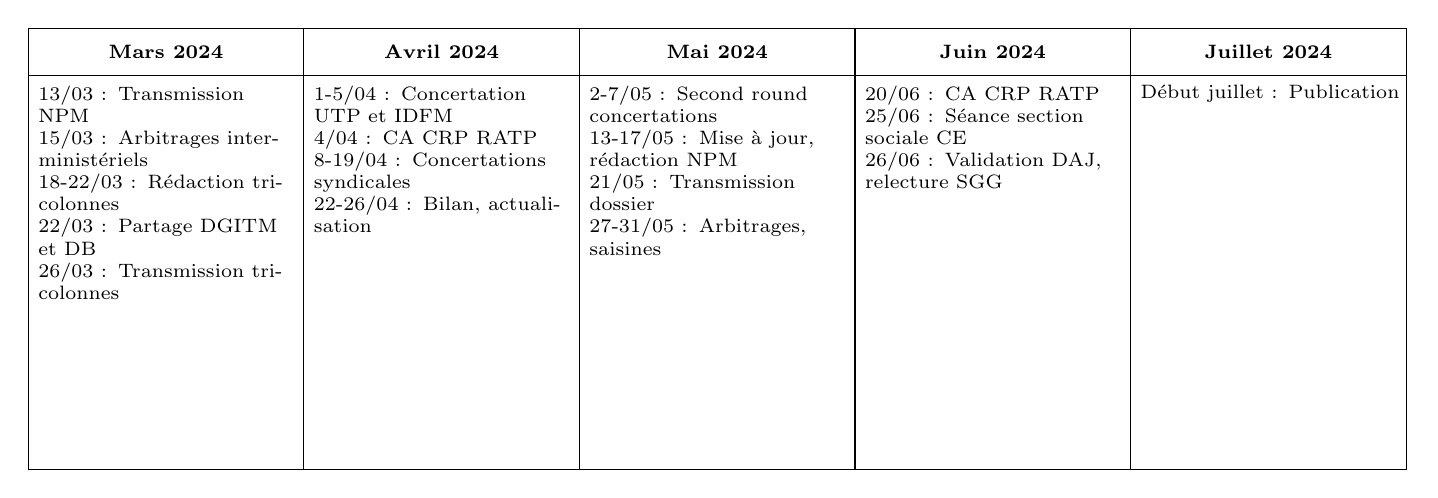
\begin{tikzpicture}[every node/.style={font=\scriptsize}]
\def\monthwidth{3.5cm}
\def\monthheight{5cm}
\def\headerheight{0.6cm}

% Macro for month column
\newcommand{\monthcolumn}[3]{
    % Header
    \draw (#1*\monthwidth,\monthheight) rectangle (#1*\monthwidth+\monthwidth,\monthheight+\headerheight);
    \node[anchor=center] at (#1*\monthwidth+0.5*\monthwidth,\monthheight+0.5*\headerheight) {\textbf{#2}};
    
    % Content
    \draw (#1*\monthwidth,0) rectangle (#1*\monthwidth+\monthwidth,\monthheight);
    \node[text width=3.3cm,anchor=north west,align=left] at (#1*\monthwidth+0.1,\monthheight-0.1) {#3};
}

% Mars 2024
\monthcolumn{0}{Mars 2024}{
    13/03 : Transmission NPM\\
    15/03 : Arbitrages interministériels\\
    18-22/03 : Rédaction tricolonnes\\
    22/03 : Partage DGITM et DB\\
    26/03 : Transmission tricolonnes
}

% Avril 2024
\monthcolumn{1}{Avril 2024}{
    1-5/04 : Concertation UTP et IDFM\\
    4/04 : CA CRP RATP\\
    8-19/04 : Concertations syndicales\\
    22-26/04 : Bilan, actualisation
}

% Mai 2024
\monthcolumn{2}{Mai 2024}{
    2-7/05 : Second round concertations\\
    13-17/05 : Mise à jour, rédaction NPM\\
    21/05 : Transmission dossier\\
    27-31/05 : Arbitrages, saisines
}

% Juin 2024
\monthcolumn{3}{Juin 2024}{
    20/06 : CA CRP RATP\\
    25/06 : Séance section sociale CE\\
    26/06 : Validation DAJ, relecture SGG
}

% Juillet 2024
\monthcolumn{4}{Juillet 2024}{
    Début juillet : Publication
}

\end{tikzpicture}
}
        \caption{Calendrier de travail du bureau 3B}\label{fig:retroplanning}
\end{figure}


  \subsubsection{Les enjeux de la réforme}

Pour le bureau 3B et 3C qui élabore cette réforme, les enjeux sont multiples :
\begin{itemize}
    \item Adapter la complexité du régime spécial de retraite afin de proposer un dispositif clair pour les nouveaux employeurs habitués au régime général.
    \item Éviter des effets gagnants/perdants parmi les salariés transférés.
    \item Rester en lien étroit avec les partenaires sociaux de la RATP pour s'assurer de l'acceptabilité sociale des mesures prises.
\end{itemize}

   
%----------------------------------------------------------------------------------------
%	SECTION 2
%----------------------------------------------------------------------------------------
\clearpage 

\section{Comparaison entre le regime spécial de la RATP et le regime général}

\subsection{Structure de l'emploi, de la rémunération et des droits associés}

Bien que les agents de la RATP soient des salariés de droit privé, ils sont néanmoins des salariés à statut. Cela ne signifie pas pour autant que ce sont des fonctionnaires.

Les explications que l'on trouve sur le site internet du Ministère de la Transition écologique et de la Cohésion des territoires sont particulièrement intéressantes :
\\
\textit{\\Ces statuts du personnel ont pour objet de prévoir notamment les conditions de recrutement et de cessation de fonctions, la rémunération, les congés de tout nature, certains droits syndicaux, les garanties disciplinaires. Ils sont élaborés au sein des établissements publics après consultation des organisations syndicales et font l’objet d’une approbation ministérielle. Ils revêtent la qualité d’actes réglementaires dont la légalité est soumise à l’appréciation du juge administratif.\\
Historiquement, la mise en place du statut dans les années 50 s’expliquait par la volonté d’exclure les entreprises publiques du champ de la négociation collective.
En vertu des dispositions de la loi du 11 février 1950 relative aux conventions collectives, les relations collectives de travail dans certaines entreprises et établissements du secteur public n’étaient pas déterminées par voie d’accord négocié, mais faisaient l’objet d’un statut législatif ou réglementaire. La loi fondait ainsi une exclusion réciproque entre accords collectifs et statuts de personnel.}

Ainsi, bien que les agents RATP ne soient pas des fonctionnaires, le fonctionnement de leurs rémunération s'inspire beaucoup de celui de la fonction publique.

Elle est composée d'un traitement indiciaire qui augmente avec l'ancienneté. Et de primes, qui elles sont versées en fonctions du travail ou des conditions de travail d'un agent. Il existe par exemple des primes de travail sur jours fériés, ou encore des primes pour conduite sans accident qui augmente avec le nombre de kilomètre parcouru sans accident.

Pour les salariés de droits communs, la rémunération est un salaire, encadré par les accords de branches. Il peut être négocié individuellement au moment de l'embauche. Une part du salaire peut également être variables et comprendre des primes.


\subsection{Assiette sociale et taux de cotisations}

Outre la structure des rémunérations, une des différences majeures entre le régime de la RATP et le régime générale se trouve au niveau des taux et assiettes de cotisations.
L'assiette de cotisation du régime spéciale de la RATP ne comprend pas l’ensemble des éléments de rémunération des salariés (en particulier, la plupart des primes). Alors que l'assiette de cotisation du RG comprend l'ensemble des éléments de rémunération.
Quant au taux de cotisation, il se décompose entre d’une part, le taux de cotisation salarial qui est supérieur à celui du régime général et s’établit à 12,95 \%, et d’autre part, le taux de cotisation patronal de 19,19 \% qui est révisé chaque année de telle sorte que la masse des cotisations soit équivalente à celle qui aurait été versée par l’employeur RATP si le régime avait été adossé au régime général. En pratique, le taux de cotisations à la charge de la Régie fait l’objet chaque année d’un arrêté fixant un taux de cotisations provisionnel pour l’année en cours qui devient définitif l’année suivante ; ce taux fait l’objet de régularisation afin de correspondre, en montant, à ce que la Régie aurait versé si ses salariés avaient relevé du régime général. Pour l’exercice 2022, le taux définitif de la cotisation à la charge de la RATP était fixé à 19,19 \%, tandis que le taux provisionnel de la cotisation à la charge de la RATP était fixé à 19,13 \% pour l’exercice 2023.  

Le calcul des droits à la retraite se fait également différemment. Comme pour les fonctionnaires, la pension à taux plein est égale à 75 \% du salaire (hors primes) des 6 derniers mois. Tandis que pour les salariés de droit communs la pension à taux plein est égale à 50 \% du salaire des 25 années les plus avantageuses de leurs carrière.


\subsection{Contrainte de la réforme : sauvegarde des droits futurs et de la rémunération}

En plus de toutes ces spécificités du régime de la RATP à prendre en compte lors du transfert des agents, l’article L. 3111-16-7 du code des transports a inscrit le principe d’une garantie de rémunération en cas de changement d’employeur des salariés RATP transférés dans le cadre de l’ouverture à la concurrence. Il est ainsi prévu que le niveau de rémunération des salariés transférés ne peut être inférieur au montant annuel, pour une durée de travail équivalente, des éléments de rémunération (traitement et primes), hors éléments exceptionnels, versés lors des douze mois précédant la date de changement effectif d’employeur. L’article précise que la garantie porte sur la rémunération nette de cotisations salariales. En pratique, le nouvel employeur verse au salarié une indemnité différentielle pour garantir son niveau de rémunération. Cette indemnité diminue en fonction des augmentations de salaire obtenues par le salarié après le transfert. En résumé, l'indemnité différentielle compense la perte de rémunération engendrée par le changement d’employeur.


%----------------------------------------------------------------------------------------
%	SECTION 3
%----------------------------------------------------------------------------------------
\clearpage 

\section{Mise en place du sac-à-dos Social}

\subsection{Alignement des cotisations pour les salariés transférés}

Afin de déterminer les taux et assiettes de cotisations applicables aux salariés transférés, deux scénarios ont été envisagés.
Soit l’application des taux et de l’assiette de cotisations sociales du régime général, soit le maintien des taux du régime spécial appliquée à une assiette de cotisations sociales reconstituée. Si ces scénarios sont neutres par construction pour la part patronale, leurs effets diffèrent sensiblement pour la part salariale. Pour le « sac à dos social » SNCF, l'option qui avait était privilégie était d’appliquer les taux de cotisations salarial et patronal du régime spécial de la SNCF aux salariés transférés et aux futurs employeurs sur la base d’une assiette de cotisations abattue afin de reconstituer l’assiette de cotisations du régime spécial.  

Dans le détail, le premier scénario consiste à appliquer les taux et l’assiette de cotisations salariale et patronale du régime général et du régime AGIRC-ARRCO sur la rémunération des salariés transférés. L’application des taux de droit commun présente une meilleure lisibilité et une simplicité de mise en œuvre pour les employeurs. Un seul système de cotisations existerait avec une implémentation facilitée, notamment d’un point de vue déclaratif dans les systèmes d’information (DSN notamment).
Ce scénario présente toutefois une difficulté juridique au regard du principe d’égalité devant les charges publiques. En effet, les salariés transférés continueront de bénéficier des pensions et prestations – modulo les adaptations nécessaires pour tenir compte du changement d’employeur – du régime spécial de retraite de la RATP tout en cotisant avec des taux différents de ceux des salariés statutaires. De plus ce scénario créerait de fortes distorsions entre les salariés compte tenu de la forte variabilité de
la part des éléments non-cotisables dans leur rémunération, rendant peu justifiable la dérogation au principe d’égalité devant les charges publiques. 

Par exemple, un cadre du réseau de surface transféré, dont la rémunération comporte peu de primes non cotisables, verserait moins de cotisations sociales (- 4 383 €) du fait de la baisse du taux de cotisations alors qu’un machiniste receveur de grade BC2, dont la rémunération statutaire est composée de nombreuses primes non cotisables, devrait cotiser après son transfert sur la totalité de sa rémunération (+ 5 652 €).

L’option alternative consisterait à maintenir les taux de cotisations sociales du régime spécial sur les rémunérations des salariés transférés.  L’application des taux de cotisations du régime spécial suppose de reconstituer l’assiette de cotisations sociales sur le modèle de l’assiette du régime spécial afin de reprendre la part des éléments cotisables et ceux non-cotisables dans la rémunération totale. 

Dans ce objectif, deux solutions ont été envisagées : 
\begin{itemize}
    \item application d’un coefficient d’abattement par groupements d’emplois : au moment du transfert, l’agent se verrait appliquer un coefficient d’abattement, défini en fonction de son emploi, sur sa rémunération. La liste des coefficients d’abattement serait définie par arrêté en fonction du type d’emploi, de sorte qu’en cas de changement d’emploi, le salarié se verrait appliquer un nouveau coefficient d’abattement pour la reconstitution de son assiette de cotisations ;
    \item exclusion de l’assiette de cotisations des éléments non cotisables : un arrêté fixerait la liste des éléments non cotisables (primes) en cohérence avec la structure de rémunération des salariés statutaires : l’assiette ainsi reconstituée serait individualisée et évolutive.
\end{itemize}

Pour la première solution, des coefficients d’abattement devraient être déterminés pour reconstituer l’assiette de cotisations. Le coefficient appliqué serait celui correspondant au métier exercé au moment du transfert, sans possibilité d’actualisation des coefficients car, contrairement au modèle SNCF, l’ensemble des métiers concernés par l’ouverture à la concurrence ont vocation à être transférés.

J'ai donc été chargé d'explorer les différentes manières de calculer un coefficient d'abattement permettant de reconstituer l'assiette de cotisation. C'est un travail de résolution d'équation qui fut long mais très intéressant et que je vais détailler ci dessous :


Pour commencer, mes variables sont : \\
Coefficient pour égaliser les assiettes : \(X\) \\
Rémunération RATP : \(Rem_{RATP} = RI + Primes\) \\
Cotisation RATP : \(Cotis_{RATP} = RI \times tx_{RATP}\) \\
Rémunération après transfert : \(Rem_{post-transfert}\) \\
Cotisation au RG : \(Cotis_{RG} = (RI + Primes) \times tx_{RG}\) \\
\\
On veut que la rémunération nette après transfert soit supérieure ou égale à la rémunération nette. \\
On a donc : 
\[
Rem_{post-transfert} - Cotis_{RG} \geq Rem_{RATP} - Cotis_{RATP}
\]
On pose notre équation comme suit : 
\begin{multline*}
Rem_{RATP} - (RI \times tx_{RATP}) = Rem_{post-transfert} \\
- (RI + Primes) \times tx_{RG} \times X \\
\end{multline*}
\text{Ici, les deux rémunérations s'annulent et on a donc :} \\
\begin{align*}
- RI \times tx_{RATP} &= - (RI + Primes) \times tx_{RG} \times X\\
X &= \frac{RI \times tx_{RATP}}{(RI + Primes) \times tx_{RG}} 
\end{align*}


Ce résultat est finalement assez intuitif. Le coefficient permettant de reconstruire l'assiette est le rapport des cotisations à la RATP sur les cotisations post-transfert. Ce coefficient permet d'égaliser parfaitement les rémunération avant et après transfert, mais pour des problématiques de système d'information, cette solution de coefficient individuel n'a pas pu être retenu. J'ai ensuite réaliser différents tests avec des coefficients moyen et médian par catégorie d'emploi mais les résultats n'ont pas été très satisfaisant. En effet les situations dans une catégorie d'emploi était trop variable et l'application de coefficient moyen ou médian créer de fortes inégalités.

Nous avons donc décidé d'abandonner cette piste. De plus, il était important que le coefficient et l'indemnité différentielle apparaissent tout deux dans l'équation. J'ai donc recommencer le travail avec ces deux inconnus. Je recommence donc le travail en posant l'équation comme cela :
\begin{equation*}
Rem_{RATP} - Cotis_{RATP} = Rem_{post-transfert} + ID - (X \times tx_{RG} \times (Assiette + ID))\\
\end{equation*}
\\
\text{Je ne détaillerais pas les calculs qui sont un peu longs mais on aboutit aux deux valeurs suivantes :} \\
\begin{multline*}
X = \frac{Cotis_{RATP}}{(Rem_{post-transfert} + ID) \times tx_{RATP}}\\
\\
ID = \frac{Cotis_{RATP}}{X \times tx_{RATP}} \min Rem_{post-transfert}
\end{multline*}


Ici, on aboutit à une solution ou le coefficient et l'indemnité différentielle sont inter dépendant. Si on veut augmenter l'indemnité différentielle jusqu'à un certain niveau, on doit également modifié X, ce qui fait baisser ID, on doit donc réaugmenter ID au niveau souhaitez etc.

Finalement ce scénario qui avait été retenu dans le cadre du sac à dos social SNCF, a été rejeté par la RATP dans la mesure  où la structure de rémunération de la RATP induit de fortes disparités entre agents appartenant à une même  catégorie d’emploi. En outre, contrairement à la branche ferroviaire, il ne sera pas possible de faire évoluer régulièrement le niveau des coefficients d’abattement dans la mesure où il  est prévu de transférer la quasi-intégralité des salariés de la RATP à terme.

Par conséquent, c'est le second scénario qui a été choisi. Il nécessite néanmoins de définir suffisamment précisément la  liste des éléments non cotisables afin de limiter le risque d’effet d’aubaine pour les employeurs qui pourraient être  incités à augmenter la part de ces éléments dans la rémunération pour réduire l’assiette cotisable. 

Concrètement, ce travail consiste à répertorier de manière exhaustive les primes RATP non cotisables que les salariés transférés auraient pu percevoir ou continuer à percevoir à l’EPIC en l’absence de transfert puis à transposer ces primes non cotisables en primes du droit commun, en leur attribuant une dénomination et des conditions d’obtention analogues et ne souffrant aucune ambiguïté.


\subsection{Avenir de la réforme}

L'arbitrage de Matignon sur le périmètre de transposition des primes ayant était rendu avant la dissolution, le travail de rédaction des textes juridiques a pu être finalisé cet été.
Une concertation avec les organisations syndicales, patronales, certaines entreprises candidates et la RATP a pu être menée.

Les premiers décrets ont pu être soumis au Conseil d'Etat fin août et les arrêtes sont eux en cours de validation en interne.

Cette mission a été très intéressante pour plusieurs raison. Elle m'a permit d'assister en direct à l'élaboration de mesures politiques particulièrement sensibles. J'ai pu travailler en collaboration avec un grand nombre d'acteurs institutionnels ou du secteur du transport. Cette mission m'a également permis de faire face aux difficultés inhérentes à ce type de travaux. De nombreuses possibilités doivent être explorées même si elles ne sont finalement pas adoptées. 

			%2 - Conclusion

%Gros travail sur le scénario avec détermination d'au taux

%#### Equation de détermination du coef d'abbatement

%####  Chiffagres individuels, par moy ou med de groupe
%- tableau resume pour NPM avec cas types

%#### difficulté juridique, on opte pour la ersion avec listes de primes


\chapter{Réforme de l'assiette sociale des Travailleurs Indépendants et des Professions Libérales} % Main chapter title


Contrairement aux employeurs et aux salariés, les travailleurs indépendants (artisans, commerçants, professionnels libéraux, avocats, travailleurs non-salariés agricoles) cotisent aujourd’hui sur deux assiettes différentes selon la nature des prélèvements. L'une pour les cotisations et l'autre pour les contributions sociales (CSG et CRDS).

Ces deux assiettes sont circulaires, c’est-à-dire qu’il est nécessaire de connaître le montant des cotisations et des contributions pour déterminer l’assiette permettant de calculer ces mêmes cotisations et contributions, ce qui induit une forte complexité. 

De plus, en 2019, un rapport sur les travailleurs indépendants rendu par le Haut Conseil du Financement de 
la Protection Sociale (HCFIPS) établi que pour un euro de prélèvement social, ces derniers payent plus de CSG-CRDS et moins de cotisations que les salariés. Cette différence s'explique par le fait que l’assiette de CSG-CRDS (non créatrice de droits) soit supérieure à celle des cotisations (prise en compte pour la détermination des droits vieillesses et d’indemnités journalières). Cette situation est peu équitable vis-à-vis des salariés dont l’assiette brute, sert à la fois pour le calcul des cotisations et de la CSG-CRDS.

Afin de gommer cette injustice et dans un effort de simplification de la lisibilité du calcul des cotisations pour les affiliés, une reforme des l'assiette sociale des travailleurs indépendants et des professions libérales est en cours.
Ce chapitres à vocation à expliquer plus précisément le cadre dans lequel cette réforme a lieu, ses objectifs, et le travail que le Pôle Actuariat a réalisé pour la mener à bien.


%----------------------------------------------------------------------------------------
%	SECTION 
%----------------------------------------------------------------------------------------
\section{Paysage de la retraite en France}


\subsection{La retraite par répartition}

Le système de retraite français est construit autour de deux grands piliers.
La retraite de base et la retraite complémentaire.
La retraite de base des salariés du secteur privé, des travailleurs indépendants, des contractuels de droit public et des artistes-auteurs est gérée par la Caisse National d'Assurance Vieillesse (CNAV). La retraite de base des professionnels libéraux est gérée par la Caisse nationale d'assurance vieillesse des professions libérales (CNAVPL).
Les régimes complémentaires des professions libérales sont gérées par les 10 sections professionnelles.

Tous ces régimes de retraite sont gérés par répartition, c'est à dire que les cotisations des travailleurs actifs servent à financer les pensions des retraités. Chaque génération d'actifs cotise pour payer les retraites des générations précédentes, ce qui repose sur un principe de solidarité intergénérationnelle. 

Aujourd'hui, le système de retraite fait face à de nombreux défis. Le vieillissement de la population, avec l'allongement de l'espérance de vie et le départ à la retraite des baby-boomers, met sous pression l'équilibre du financement. Le taux de cotisation des actifs doit augmenter ou le montant des pensions doit baisser pour compenser cette évolution, à moins d'augmenter l'âge de départ à la retraite. Ces enjeux poussent à des réformes régulières.

Les dernières réformes des retraites, comme celle de 2023 en France, ont principalement visé à repousser l'âge légal de départ à la retraite (de 62 à 64 ans), à allonger la durée de cotisation pour obtenir une pension complète, et à harmoniser certains régimes. Ces réformes cherchent à garantir la pérennité du système en équilibrant les dépenses et les recettes, tout en tenant compte de l'évolution démographique. Les débats autour des retraites restent vifs, notamment sur la justice sociale et la répartition des efforts entre les différentes catégories de la population.

\subsection{Les régimes de base des TI et PL}

La Caisse nationale d'assurance vieillesse des professions libérales (CNAVPL) a été créée pour répondre aux besoins spécifiques de retraite des professionnels exerçant des métiers indépendants. Fondée en 1948, elle regroupe dix sections professionnelles couvrant diverses catégories, comme les médecins, dentistes, pharmaciens, avocats, experts-comptables, vétérinaires, etc. La CNAVPL gère le régime de base des libéraux, communs à toutes les sections, tandis que celles-ci ont la responsabilité de gérer leurs propres régime complémentaire, adapté aux particularités économiques et professionnelles de ses affiliés. Le système fonctionne par répartition, où les cotisations des actifs financent les pensions des retraités.

La CNBF a été une section de sa création de 1948 à sa transformation en organisme autonome en 1954.

Le règime de la CNAVPL est un régime par point, ce qui est assez rare pour un régime de base. Au 30 juin 2023, la CNAVPL a, 880 000 cotisants, 425 000 retraités et 53 000 conjoints survivants bénéficiant d'une pension de réversion. La cotisation se calcule comme suit. Une cotisation de 8,23 \% est prélevée sur la part du revenu annuel située en dessous du plafond de la Sécurité sociale (PASS). Une cotisation de 1,87 \% est prélevée sur la part du revenu annuel située en dessous de 5 PASS.
En pratique, un affilié cotise donc 10,10 \% (8,23 \% + 1,87 \%) jusqu'au PASS et 1,87 \% entre 1 et 5 PASS.


\subsection{Les régimes de complémentaires des TI et PL}

Tous d'abord, voilà la liste des caisses de la CNAVPL ainsi que la profession de leurs affiliés.

\begin{itemize}
    \item \textbf{Les dix sections de la CNAVPL :}
    \begin{itemize}
        \item \textbf{CARCDSF} : chirurgiens-dentistes et sages-femmes
        \item \textbf{CARMF} : médecins
        \item \textbf{CARPIMKO} : infirmiers, masseurs-kinesithérapeutes, pédicures-podologues, orthophonistes et orthoptistes
        \item \textbf{CARPV} : vétérinaires
        \item \textbf{CAVAMAC} : agents généraux d’assurance
        \item \textbf{CAVEC} : experts-comptables
        \item \textbf{CAVOM} : officiers ministériels, officiers publics et des compagnies judiciaires
        \item \textbf{CAVP} : pharmaciens
        \item \textbf{CIPAV} : architectes, architectes d’intérieur, économistes de la construction, maîtres d’œuvre, géomètres, ingénieurs conseils, moniteurs de ski, guides de haute montagne, accompagnateurs de moyenne montagne, ostéopathes, psychologues, psychothérapeutes, ergothérapeutes, diététiciens, chiropracteurs, artistes non créateurs d’œuvres originales, experts en automobile, experts devant les tribunaux, guides conférenciers, mandataires judiciaires à la protection des majeurs
        \item \textbf{CPRN} : notaires
    \end{itemize}
\end{itemize}

Entre les différentes professions libérales, le panorama des barèmes de cotisations et prestations est caractérisé par une grande diversité. En effet, si le régime de base de retraite est commun à l’ensemble des professions libérales, chacune des sections composant la CNAVPL dispose d’un régime complémentaire propre et éventuellement d’un régime « sur-complémentaire » de prestations complémentaire de vieillesse dit PCV (anciennement « avantage social vieillesse » ou ASV) pour les sections médicales. Chaque section gère également un régime d’invalidité-décès.

Les régimes de retraite et d’invalidité-décès peuvent sensiblement varier au sein d’une même section. C’est par exemple le cas pour la CARCDSF, qui regroupe depuis 2009 les chirurgiens-dentistes et sages-femmes, et dont le régime PCV est distinct selon la profession. Il existe également des divergences au sein d’une même profession : par exemple les médecins de secteur 1 bénéficient d’une participation des assurances maladie, notamment sur leurs cotisations du régime de base et du régime PCV, à la différence de leurs confrères du secteur 2. Cette différence sera détaillé dans un exemple plus bas.

%----------------------------------------------------------------------------------------
%	SECTION 
%----------------------------------------------------------------------------------------
\section{Contexte et objectifs de la réforme}
\label{sec:2.2}

\subsection{Le fonctionnement de l'assiette aujourd'hui}

Pour bien comprendre la circularité du calcul de l'assiette actuelle, il est nécessaire de bien comprendre la décomposition du \textbf{Superbrut}. Le superbrut est un concept utilisé pour désigner le salaire comprenant non seulement les cotisations salariales (qui sont déduites du salaire brut classique), mais aussi l'ensemble des cotisations patronales. Dans le cas des travailleurs indépendants ou des professions libérales, le concept de superbrut s'applique différemment. Ces travailleurs ne perçoivent pas de salaire brut comme les salariés, car ils sont à la fois employeur et salarié de leur propre activité. Ils doivent donc payer l'intégralité des cotisations sociales (à la fois la part "salariale" et la part "patronale") sur leurs revenus professionnels. La figure ci-dessous reproduit cette décomposition par strates de prélèvement.  

\vspace{0.2cm}

\begin{figure}[!h]
    \center
    %créer avec https://www.mathcha.io/
\tikzset{
pattern size/.store in=\mcSize, 
pattern size = 5pt,
pattern thickness/.store in=\mcThickness, 
pattern thickness = 0.3pt,
pattern radius/.store in=\mcRadius, 
pattern radius = 1pt}
\makeatletter
\pgfutil@ifundefined{pgf@pattern@name@_1xrvl3kqi}{
\pgfdeclarepatternformonly[\mcThickness,\mcSize]{_1xrvl3kqi}
{\pgfqpoint{0pt}{0pt}}
{\pgfpoint{\mcSize+\mcThickness}{\mcSize+\mcThickness}}
{\pgfpoint{\mcSize}{\mcSize}}
{
\pgfsetcolor{\tikz@pattern@color}
\pgfsetlinewidth{\mcThickness}
\pgfpathmoveto{\pgfqpoint{0pt}{0pt}}
\pgfpathlineto{\pgfpoint{\mcSize+\mcThickness}{\mcSize+\mcThickness}}
\pgfusepath{stroke}
}}
\makeatother

% Pattern Info
 
\tikzset{
pattern size/.store in=\mcSize, 
pattern size = 5pt,
pattern thickness/.store in=\mcThickness, 
pattern thickness = 0.3pt,
pattern radius/.store in=\mcRadius, 
pattern radius = 1pt}
\makeatletter
\pgfutil@ifundefined{pgf@pattern@name@_j0bpecchi}{
\pgfdeclarepatternformonly[\mcThickness,\mcSize]{_j0bpecchi}
{\pgfqpoint{-\mcThickness}{-\mcThickness}}
{\pgfpoint{\mcSize}{\mcSize}}
{\pgfpoint{\mcSize}{\mcSize}}
{
\pgfsetcolor{\tikz@pattern@color}
\pgfsetlinewidth{\mcThickness}
\pgfpathmoveto{\pgfpointorigin}
\pgfpathlineto{\pgfpoint{0}{\mcSize}}
\pgfusepath{stroke}
}}
\makeatother

% Pattern Info
 
\tikzset{
pattern size/.store in=\mcSize, 
pattern size = 5pt,
pattern thickness/.store in=\mcThickness, 
pattern thickness = 0.3pt,
pattern radius/.store in=\mcRadius, 
pattern radius = 1pt}
\makeatletter
\pgfutil@ifundefined{pgf@pattern@name@_lqqskltm4}{
\makeatletter
\pgfdeclarepatternformonly[\mcRadius,\mcThickness,\mcSize]{_lqqskltm4}
{\pgfpoint{-0.5*\mcSize}{-0.5*\mcSize}}
{\pgfpoint{0.5*\mcSize}{0.5*\mcSize}}
{\pgfpoint{\mcSize}{\mcSize}}
{
\pgfsetcolor{\tikz@pattern@color}
\pgfsetlinewidth{\mcThickness}
\pgfpathcircle\pgfpointorigin{\mcRadius}
\pgfusepath{stroke}
}}
\makeatother

% Gradient Info
  
\tikzset {_52ujinwbo/.code = {\pgfsetadditionalshadetransform{ \pgftransformshift{\pgfpoint{0 bp } { 0 bp }  }  \pgftransformrotate{0 }  \pgftransformscale{2 }  }}}
\pgfdeclarehorizontalshading{_8zfhmi56e}{150bp}{rgb(0bp)=(1,1,1);
rgb(37.5bp)=(1,1,1);
rgb(50bp)=(0.95,0.95,0.95);
rgb(50.25bp)=(0.93,0.93,0.93);
rgb(62.5bp)=(1,1,1);
rgb(100bp)=(1,1,1)}
\tikzset{every picture/.style={line width=0.75pt}} %set default line width to 0.75pt        

\begin{tikzpicture}[x=0.75pt,y=0.75pt,yscale=-1,xscale=1]
%uncomment if require: \path (0,323); %set diagram left start at 0, and has height of 323

%Shape: Rectangle [id:dp3289677688045156] 
\draw  [color={rgb, 255:red, 0; green, 0; blue, 0 }  ,draw opacity=1 ][pattern=_1xrvl3kqi,pattern size=6pt,pattern thickness=0.75pt,pattern radius=0pt, pattern color={rgb, 255:red, 0; green, 0; blue, 0}] (225.6,17.61) -- (349,17.61) -- (349,93.71) -- (225.6,93.71) -- cycle ;
%Shape: Rectangle [id:dp8682136248456864] 
\draw  [pattern=_j0bpecchi,pattern size=6pt,pattern thickness=0.75pt,pattern radius=0pt, pattern color={rgb, 255:red, 0; green, 0; blue, 0}] (225.6,95) -- (349,95) -- (349,137) -- (225.6,137) -- cycle ;
%Shape: Rectangle [id:dp40966310157166896] 
\draw  [pattern=_lqqskltm4,pattern size=6pt,pattern thickness=0.75pt,pattern radius=0.75pt, pattern color={rgb, 255:red, 0; green, 0; blue, 0}] (225.6,137.54) -- (349,137.54) -- (349,161) -- (225.6,161) -- cycle ;
%Shape: Rectangle [id:dp5739807656638256] 
\path  [shading=_8zfhmi56e,_52ujinwbo] (225.6,161.02) -- (349.3,160.98) -- (349.35,310.07) -- (225.65,310.11) -- cycle ; % for fading 
 \draw   (225.6,161.02) -- (349.3,160.98) -- (349.35,310.07) -- (225.65,310.11) -- cycle ; % for border 

%Shape: Right Angle [id:dp28002043459513914] 
\draw  [line width=1.5]  (358.22,137.54) -- (364.9,137.54) -- (364.9,308) ;
%Straight Lines [id:da8011051611987892] 
\draw [line width=1.5]    (355.99,308) -- (364.9,308) ;
\draw   (373.82,195.98) -- (392.77,202.68) -- (373.82,209.38) -- (383.29,202.68) -- cycle ;
%Shape: Right Angle [id:dp10347333051497687] 
\draw  [dash pattern={on 1.69pt off 2.76pt}][line width=1.5]  (220.11,17) -- (214.45,17) -- (214.45,308) ;
%Straight Lines [id:da6254790804259747] 
\draw [line width=1.5]  [dash pattern={on 5.63pt off 4.5pt}]  (215.48,308) -- (220.11,308) ;

% Text Node
\draw (234.06,214.29) node [anchor=north west][inner sep=0.75pt]  [font=\large] [align=left] {{\fontfamily{pcr}\selectfont \textbf{Revenu net}}};
% Text Node
\draw (263.78,141.5) node [anchor=north west][inner sep=0.75pt]  [font=\footnotesize] [align=center] {{\fontfamily{pcr}\selectfont \textbf{CSG ND}}};
% Text Node
\draw (241.12,106.84) node [anchor=north west][inner sep=0.75pt]  [font=\footnotesize] [align=left] {{\fontfamily{pcr}\selectfont \textbf{{\small CSG Déductib}le}}};
% Text Node
\draw (235.37,44.64) node [anchor=north west][inner sep=0.75pt]  [font=\footnotesize] [align=left] {};
% Text Node
\draw (247.89,36.96) node [anchor=north west][inner sep=0.75pt]  [font=\footnotesize] [align=left] {\begin{minipage}[lt]{51.67pt}\setlength\topsep{0pt}
\begin{center}
{\fontfamily{pcr}\selectfont \textbf{Cotisations }}\\{\fontfamily{pcr}\selectfont \textbf{sociales}}
\end{center}

\end{minipage}};
% Text Node
\draw (409.49,180.07) node [anchor=north west][inner sep=0.75pt]   [align=left] {\begin{minipage}[lt]{51.8pt}\setlength\topsep{0pt}
\begin{center}
{\fontfamily{pcr}\selectfont Assiette de}\\{\fontfamily{pcr}\selectfont cotisations}
\end{center}

\end{minipage}};
% Text Node
\draw (182.95,201.65) node [anchor=north west][inner sep=0.75pt]  [font=\large,rotate=-270] [align=left] {{\fontfamily{pcr}\selectfont \textbf{Superbrut}}};


\end{tikzpicture}
 %créer avec https://www.mathcha.io/
    \caption{Décomposition du Super-Brut}
\end{figure}

\newpage

Le Super brut se décompose ainsi selon la formule suivante : 

\vspace{0.2cm}

\begin{equation}
\mathbf{
Superbrut = Revenu_{net} + CSG_{non-d\Acute{e}ductible} + CSG_{d\Acute{e}ductible} + Cotisations \: Sociales \label{equa_prp}
}
\end{equation}

\vspace{0.5cm}

Où l'assiette des cotisations \footnote{Cotisations sociales hors CSG-CRDS} - qui permet in-fine de calculer les cotisations sociales dues\footnote{Les cotisations de sécurité sociale dues par les travailleurs indépendants non agricoles ne relevant pas du dispositif prévu à l'article L. 613-7
sont assises sur une assiette nette constituée du montant des revenus d'activité indépendante à retenir, sous réserve des dispositions des II à IV du présent article, pour le calcul de l'impôt sur le revenu, diminuée du montant de cotisations calculé selon les modalités fixées au V. - (Articles L131-6 à L131-6-2)} - est composé du \(Revenu_{net}\) et de la \(CSG_{non-d\Acute{e}ductible}\) tel que : 

\vspace{0.2cm}

\begin{equation}
\mathbf{
Assiette_{Cotisations \: Sociales} = Revenu_{net} + CSG_{non-d\Acute{e}ductible} 
}
\end{equation}

\vspace{0.5cm}

De même pour l'assiette de cotisation de la CSG-CRDS : 

\vspace{0.2cm}

\begin{equation}\label{eq:test}
\mathbf{
Assiette_{\: CGS-CRDS} = Revenu_{net} + CSG_{non-d\Acute{e}ductible} + Cotisations \: Sociales
}
\end{equation}

\begin{equation}
\mathbf{
Assiette_{\: CGS-CRDS} = SuperBrut - CSG_{D\Acute{e}ductible} \tag{\ref{eq:test}}
}
\end{equation}

\vspace{0.2cm}

Le schéma suivant permet de comprendre la décomposition de ces deux assiettes. La présence de la CSG non-déductible  dans l'écriture des deux assiettes nous permet de matérialiser la jonction entre le Super Brut et le Revenu Net. 

\begin{figure}[!h]
    \center
    %créer avec https://www.mathcha.io/
% Pattern Info
 
\tikzset{
pattern size/.store in=\mcSize, 
pattern size = 5pt,
pattern thickness/.store in=\mcThickness, 
pattern thickness = 0.3pt,
pattern radius/.store in=\mcRadius, 
pattern radius = 1pt}
\makeatletter
\pgfutil@ifundefined{pgf@pattern@name@_ztkrxlp1t}{
\pgfdeclarepatternformonly[\mcThickness,\mcSize]{_ztkrxlp1t}
{\pgfqpoint{0pt}{0pt}}
{\pgfpoint{\mcSize+\mcThickness}{\mcSize+\mcThickness}}
{\pgfpoint{\mcSize}{\mcSize}}
{
\pgfsetcolor{\tikz@pattern@color}
\pgfsetlinewidth{\mcThickness}
\pgfpathmoveto{\pgfqpoint{0pt}{0pt}}
\pgfpathlineto{\pgfpoint{\mcSize+\mcThickness}{\mcSize+\mcThickness}}
\pgfusepath{stroke}
}}
\makeatother

% Pattern Info
 
\tikzset{
pattern size/.store in=\mcSize, 
pattern size = 5pt,
pattern thickness/.store in=\mcThickness, 
pattern thickness = 0.3pt,
pattern radius/.store in=\mcRadius, 
pattern radius = 1pt}
\makeatletter
\pgfutil@ifundefined{pgf@pattern@name@_kcr83hov1}{
\pgfdeclarepatternformonly[\mcThickness,\mcSize]{_kcr83hov1}
{\pgfqpoint{-\mcThickness}{-\mcThickness}}
{\pgfpoint{\mcSize}{\mcSize}}
{\pgfpoint{\mcSize}{\mcSize}}
{
\pgfsetcolor{\tikz@pattern@color}
\pgfsetlinewidth{\mcThickness}
\pgfpathmoveto{\pgfpointorigin}
\pgfpathlineto{\pgfpoint{0}{\mcSize}}
\pgfusepath{stroke}
}}
\makeatother

% Pattern Info
 
\tikzset{
pattern size/.store in=\mcSize, 
pattern size = 5pt,
pattern thickness/.store in=\mcThickness, 
pattern thickness = 0.3pt,
pattern radius/.store in=\mcRadius, 
pattern radius = 1pt}
\makeatletter
\pgfutil@ifundefined{pgf@pattern@name@_nbqv8nhqs}{
\makeatletter
\pgfdeclarepatternformonly[\mcRadius,\mcThickness,\mcSize]{_nbqv8nhqs}
{\pgfpoint{-0.5*\mcSize}{-0.5*\mcSize}}
{\pgfpoint{0.5*\mcSize}{0.5*\mcSize}}
{\pgfpoint{\mcSize}{\mcSize}}
{
\pgfsetcolor{\tikz@pattern@color}
\pgfsetlinewidth{\mcThickness}
\pgfpathcircle\pgfpointorigin{\mcRadius}
\pgfusepath{stroke}
}}
\makeatother

% Gradient Info
  
\tikzset {_z301w9evq/.code = {\pgfsetadditionalshadetransform{ \pgftransformshift{\pgfpoint{0 bp } { 0 bp }  }  \pgftransformrotate{0 }  \pgftransformscale{2 }  }}}
\pgfdeclarehorizontalshading{_s713ckaqj}{150bp}{rgb(0bp)=(1,1,1);
rgb(37.5bp)=(1,1,1);
rgb(50bp)=(0.95,0.95,0.95);
rgb(50.25bp)=(0.93,0.93,0.93);
rgb(62.5bp)=(1,1,1);
rgb(100bp)=(1,1,1)}

% Pattern Info
 
\tikzset{
pattern size/.store in=\mcSize, 
pattern size = 5pt,
pattern thickness/.store in=\mcThickness, 
pattern thickness = 0.3pt,
pattern radius/.store in=\mcRadius, 
pattern radius = 1pt}
\makeatletter
\pgfutil@ifundefined{pgf@pattern@name@_rl24rvnsv}{
\pgfdeclarepatternformonly[\mcThickness,\mcSize]{_rl24rvnsv}
{\pgfqpoint{0pt}{0pt}}
{\pgfpoint{\mcSize+\mcThickness}{\mcSize+\mcThickness}}
{\pgfpoint{\mcSize}{\mcSize}}
{
\pgfsetcolor{\tikz@pattern@color}
\pgfsetlinewidth{\mcThickness}
\pgfpathmoveto{\pgfqpoint{0pt}{0pt}}
\pgfpathlineto{\pgfpoint{\mcSize+\mcThickness}{\mcSize+\mcThickness}}
\pgfusepath{stroke}
}}
\makeatother

% Pattern Info
 
\tikzset{
pattern size/.store in=\mcSize, 
pattern size = 5pt,
pattern thickness/.store in=\mcThickness, 
pattern thickness = 0.3pt,
pattern radius/.store in=\mcRadius, 
pattern radius = 1pt}
\makeatletter
\pgfutil@ifundefined{pgf@pattern@name@_a3alhvrmz}{
\makeatletter
\pgfdeclarepatternformonly[\mcRadius,\mcThickness,\mcSize]{_a3alhvrmz}
{\pgfpoint{-0.5*\mcSize}{-0.5*\mcSize}}
{\pgfpoint{0.5*\mcSize}{0.5*\mcSize}}
{\pgfpoint{\mcSize}{\mcSize}}
{
\pgfsetcolor{\tikz@pattern@color}
\pgfsetlinewidth{\mcThickness}
\pgfpathcircle\pgfpointorigin{\mcRadius}
\pgfusepath{stroke}
}}
\makeatother

% Gradient Info
  
\tikzset {_bytf7xkna/.code = {\pgfsetadditionalshadetransform{ \pgftransformshift{\pgfpoint{0 bp } { 0 bp }  }  \pgftransformrotate{0 }  \pgftransformscale{2 }  }}}
\pgfdeclarehorizontalshading{_74gcksma4}{150bp}{rgb(0bp)=(1,1,1);
rgb(37.5bp)=(1,1,1);
rgb(50bp)=(0.95,0.95,0.95);
rgb(50.25bp)=(0.93,0.93,0.93);
rgb(62.5bp)=(1,1,1);
rgb(100bp)=(1,1,1)}

% Pattern Info
 
\tikzset{
pattern size/.store in=\mcSize, 
pattern size = 5pt,
pattern thickness/.store in=\mcThickness, 
pattern thickness = 0.3pt,
pattern radius/.store in=\mcRadius, 
pattern radius = 1pt}
\makeatletter
\pgfutil@ifundefined{pgf@pattern@name@_bo8siv8bd}{
\makeatletter
\pgfdeclarepatternformonly[\mcRadius,\mcThickness,\mcSize]{_bo8siv8bd}
{\pgfpoint{-0.5*\mcSize}{-0.5*\mcSize}}
{\pgfpoint{0.5*\mcSize}{0.5*\mcSize}}
{\pgfpoint{\mcSize}{\mcSize}}
{
\pgfsetcolor{\tikz@pattern@color}
\pgfsetlinewidth{\mcThickness}
\pgfpathcircle\pgfpointorigin{\mcRadius}
\pgfusepath{stroke}
}}
\makeatother

% Gradient Info
  
\tikzset {_74arfrkiv/.code = {\pgfsetadditionalshadetransform{ \pgftransformshift{\pgfpoint{0 bp } { 0 bp }  }  \pgftransformrotate{0 }  \pgftransformscale{2 }  }}}
\pgfdeclarehorizontalshading{_hyvmwz2sj}{150bp}{rgb(0bp)=(1,1,1);
rgb(37.5bp)=(1,1,1);
rgb(50bp)=(0.95,0.95,0.95);
rgb(50.25bp)=(0.93,0.93,0.93);
rgb(62.5bp)=(1,1,1);
rgb(100bp)=(1,1,1)}
\tikzset{every picture/.style={line width=0.75pt}} %set default line width to 0.75pt        

\begin{tikzpicture}[x=0.75pt,y=0.75pt,yscale=-1,xscale=1]
%uncomment if require: \path (0,362); %set diagram left start at 0, and has height of 362

%Shape: Rectangle [id:dp3289677688045156] 
\draw  [color={rgb, 255:red, 0; green, 0; blue, 0 }  ,draw opacity=1 ][pattern=_ztkrxlp1t,pattern size=6pt,pattern thickness=0.75pt,pattern radius=0pt, pattern color={rgb, 255:red, 0; green, 0; blue, 0}] (129.6,26.61) -- (253,26.61) -- (253,104.5) -- (129.6,104.5) -- cycle ;
%Shape: Rectangle [id:dp8682136248456864] 
\draw  [pattern=_kcr83hov1,pattern size=6pt,pattern thickness=0.75pt,pattern radius=0pt, pattern color={rgb, 255:red, 0; green, 0; blue, 0}] (129.6,104.5) -- (253,104.5) -- (253,149.5) -- (129.6,149.5) -- cycle ;
%Shape: Rectangle [id:dp40966310157166896] 
\draw  [pattern=_nbqv8nhqs,pattern size=6pt,pattern thickness=0.75pt,pattern radius=0.75pt, pattern color={rgb, 255:red, 0; green, 0; blue, 0}] (129.6,149.5) -- (253,149.5) -- (253,169.46) -- (129.6,169.46) -- cycle ;
%Shape: Rectangle [id:dp5739807656638256] 
\path  [shading=_s713ckaqj,_z301w9evq] (129.3,170.04) -- (253,170) -- (253.05,321.98) -- (129.35,322.02) -- cycle ; % for fading 
 \draw   (129.3,170.04) -- (253,170) -- (253.05,321.98) -- (129.35,322.02) -- cycle ; % for border 

%Straight Lines [id:da8709079288570507] 
\draw  [dash pattern={on 4.5pt off 4.5pt}]  (85,27) -- (253,26.61) ;
%U Turn Arrow [id:dp7667981700671573] 
\draw   (113,84) -- (97.04,84.08) .. controls (93.22,84.09) and (90.14,87.2) .. (90.16,91.02) -- (90.95,258.46) .. controls (90.97,262.28) and (94.08,265.35) .. (97.89,265.34) -- (102.5,265.31) -- (102.51,268.95) -- (112.79,261.24) -- (102.44,253.64) -- (102.46,257.27) -- (98.99,257.29) .. controls (98.99,257.29) and (98.99,257.29) .. (98.99,257.29) -- (98.21,92.11) .. controls (98.21,92.11) and (98.21,92.11) .. (98.21,92.11) -- (113.04,92.04) -- cycle ;
%Shape: Right Angle [id:dp40111964969717717] 
\draw  [line width=1.5]  (123,33.61) -- (118,33.61) -- (118,162) ;
%Straight Lines [id:da5989685765587895] 
\draw [line width=1.5]    (118,162) -- (123,162) ;
%Shape: Rectangle [id:dp648586665875317] 
\draw  [color={rgb, 255:red, 0; green, 0; blue, 0 }  ,draw opacity=1 ][pattern=_rl24rvnsv,pattern size=6pt,pattern thickness=0.75pt,pattern radius=0pt, pattern color={rgb, 255:red, 0; green, 0; blue, 0}] (412.6,21.61) -- (499,21.61) -- (499,79) -- (412.6,79) -- cycle ;
%Shape: Rectangle [id:dp9073739293676215] 
\draw  [pattern=_a3alhvrmz,pattern size=6pt,pattern thickness=0.75pt,pattern radius=0.75pt, pattern color={rgb, 255:red, 0; green, 0; blue, 0}] (413.6,104) -- (500,104) -- (500,118) -- (413.6,118) -- cycle ;
%Shape: Rectangle [id:dp275716880068557] 
\path  [shading=_74gcksma4,_bytf7xkna] (413.6,118) -- (499.96,117.98) -- (500,175) -- (413.64,175.02) -- cycle ; % for fading 
 \draw   (413.6,118) -- (499.96,117.98) -- (500,175) -- (413.64,175.02) -- cycle ; % for border 

%Shape: Rectangle [id:dp4106159960013047] 
\draw  [pattern=_bo8siv8bd,pattern size=6pt,pattern thickness=0.75pt,pattern radius=0.75pt, pattern color={rgb, 255:red, 0; green, 0; blue, 0}] (414.6,242) -- (501,242) -- (501,256) -- (414.6,256) -- cycle ;
%Shape: Rectangle [id:dp3568556336780553] 
\path  [shading=_hyvmwz2sj,_74arfrkiv] (414.6,256) -- (500.96,255.98) -- (501,313) -- (414.64,313.02) -- cycle ; % for fading 
 \draw   (414.6,256) -- (500.96,255.98) -- (501,313) -- (414.64,313.02) -- cycle ; % for border 

%Curve Lines [id:da7926515286232871] 
\draw    (493,14) .. controls (533,-16) and (531,188) .. (497,186) ;
%Curve Lines [id:da715083901358808] 
\draw    (494,232) .. controls (529,218) and (518,339) .. (497,324) ;
%Curve Right Arrow [id:dp3122753892094372] 
\draw  [fill={rgb, 255:red, 255; green, 255; blue, 255 }  ,fill opacity=1 ] (582,193.9) .. controls (582,147.95) and (560.06,110.7) .. (533,110.7) -- (533,96) .. controls (560.06,96) and (582,133.25) .. (582,179.2) ;\draw  [fill={rgb, 255:red, 255; green, 255; blue, 255 }  ,fill opacity=1 ] (582,179.2) .. controls (582,213.32) and (569.91,242.64) .. (552.6,255.48) -- (552.6,250.58) -- (533,269.75) -- (552.6,275.08) -- (552.6,270.18) .. controls (569.91,257.34) and (582,228.02) .. (582,193.9)(582,179.2) -- (582,193.9) ;
%Curve Left Arrow [id:dp24665839398946043] 
\draw  [fill={rgb, 255:red, 255; green, 255; blue, 255 }  ,fill opacity=1 ] (357,178.4) .. controls (357,228.99) and (378.04,270) .. (404,270) -- (404,255.9) .. controls (378.04,255.9) and (357,214.89) .. (357,164.3) ;\draw  [fill={rgb, 255:red, 255; green, 255; blue, 255 }  ,fill opacity=1 ] (357,164.3) .. controls (357,126.74) and (368.6,94.46) .. (385.2,80.32) -- (385.2,75.62) -- (404,79.75) -- (385.2,99.12) -- (385.2,94.42) .. controls (368.6,108.56) and (357,140.84) .. (357,178.4)(357,164.3) -- (357,178.4) ;
\draw   (279,133) -- (328.32,149.5) -- (281.36,166)(283,133) -- (332.32,149.5) -- (285.36,166) ;

% Text Node
\draw (138.06,223.29) node [anchor=north west][inner sep=0.75pt]  [font=\large] [align=left] {{\fontfamily{pcr}\selectfont \textbf{Revenu net}}};
% Text Node
\draw (162.78,153.5) node [anchor=north west][inner sep=0.75pt]  [font=\footnotesize] [align=left] {{\fontfamily{pcr}\selectfont \textbf{CSG ND}}};
% Text Node
\draw (145.12,115.84) node [anchor=north west][inner sep=0.75pt]  [font=\footnotesize] [align=left] {{\fontfamily{pcr}\selectfont \textbf{{\small CSG Déductib}le}}};
% Text Node
\draw (139.37,53.64) node [anchor=north west][inner sep=0.75pt]  [font=\footnotesize] [align=left] {};
% Text Node
\draw (151.89,45.96) node [anchor=north west][inner sep=0.75pt]  [font=\footnotesize] [align=left] {\begin{minipage}[lt]{51.67pt}\setlength\topsep{0pt}
\begin{center}
{\fontfamily{pcr}\selectfont \textbf{Cotisations }}\\{\fontfamily{pcr}\selectfont \textbf{sociales}}
\end{center}

\end{minipage}};
% Text Node
\draw (57.45,6.15) node [anchor=north west][inner sep=0.75pt]  [font=\small] [align=left] {{\fontfamily{pcr}\selectfont \textbf{Superbrut}}};
% Text Node
\draw (10.49,133.07) node [anchor=north west][inner sep=0.75pt]  [font=\normalsize] [align=left] {\begin{minipage}[lt]{53.69pt}\setlength\topsep{0pt}
\begin{center}
{\fontfamily{pcr}\selectfont {\footnotesize à retrancher }}\\{\fontfamily{pcr}\selectfont {\footnotesize pour le calcul }}\\{\fontfamily{pcr}\selectfont {\footnotesize du revenu net}}
\end{center}

\end{minipage}};
% Text Node
\draw (427.08,136.48) node [anchor=north west][inner sep=0.75pt]  [font=\scriptsize] [align=left] {{\fontfamily{pcr}\selectfont \textbf{Revenu net}}};
% Text Node
\draw (438.8,104.63) node [anchor=north west][inner sep=0.75pt]  [font=\tiny] [align=left] {{\fontfamily{pcr}\selectfont \textbf{CSG ND}}};
% Text Node
\draw (421.89,34.96) node [anchor=north west][inner sep=0.75pt]  [font=\scriptsize] [align=left] {\begin{minipage}[lt]{45.55pt}\setlength\topsep{0pt}
\begin{center}
{\fontfamily{pcr}\selectfont \textbf{Cotisations }}\\{\fontfamily{pcr}\selectfont \textbf{sociales}}
\end{center}

\end{minipage}};
% Text Node
\draw (429.08,275.48) node [anchor=north west][inner sep=0.75pt]  [font=\scriptsize] [align=left] {{\fontfamily{pcr}\selectfont \textbf{Revenu net}}};
% Text Node
\draw (439.8,241.63) node [anchor=north west][inner sep=0.75pt]  [font=\tiny] [align=left] {{\fontfamily{pcr}\selectfont \textbf{CSG ND}}};
% Text Node
\draw (526,37.07) node [anchor=north west][inner sep=0.75pt]  [font=\small] [align=left] {\begin{minipage}[lt]{52.02pt}\setlength\topsep{0pt}
\begin{center}
{\fontfamily{pcr}\selectfont \textbf{{\small Assiette }}}\\{\fontfamily{pcr}\selectfont \textbf{{\small CSG-CRDS}}}
\end{center}

\end{minipage}};
% Text Node
\draw (523,283.07) node [anchor=north west][inner sep=0.75pt]  [font=\normalsize] [align=left] {\begin{minipage}[lt]{54.86pt}\setlength\topsep{0pt}
\begin{center}
{\fontfamily{pcr}\selectfont {\small \textbf{Assiette }}}\\{\fontfamily{pcr}\selectfont {\small \textbf{cotisations }}}\\{\fontfamily{pcr}\selectfont {\small \textbf{sociales}}}
\end{center}

\end{minipage}};
% Text Node
\draw (290,239) node [anchor=north west][inner sep=0.75pt]   [align=left] {\begin{minipage}[lt]{57.08pt}\setlength\topsep{0pt}
\begin{center}
{\fontfamily{pcr}\selectfont {\scriptsize Nécessaire }}\\{\fontfamily{pcr}\selectfont {\scriptsize pour le calcul }}\\{\fontfamily{pcr}\selectfont {\scriptsize de la CSG-CRDS}}\\
\end{center}

\end{minipage}};
% Text Node
\draw (578,82) node [anchor=north west][inner sep=0.75pt]   [align=left] {\begin{minipage}[lt]{8.67pt}\setlength\topsep{0pt}
\begin{center}
\\
\end{center}

\end{minipage}};
% Text Node
\draw (585,82) node [anchor=north west][inner sep=0.75pt]   [align=left] {\begin{minipage}[lt]{50.39pt}\setlength\topsep{0pt}
\begin{center}
{\fontfamily{pcr}\selectfont {\scriptsize Nécessaire }}\\{\fontfamily{pcr}\selectfont {\scriptsize pour le calcul }}\\{\fontfamily{pcr}\selectfont {\scriptsize des cotisations }}\\{\scriptsize {\fontfamily{pcr}\selectfont sociales}}\\
\end{center}

\end{minipage}};


\end{tikzpicture}

    \caption{Décomposition des deux assiettes circulaires}
\end{figure}



\subsection{Conception administrative de la réforme de l'assiette}

Dans son rapport de 2019, le HCFIPS a proposé une réforme de l'assiette en vue d'augmenter l'assiette de cotisations et de baisser l'assiette de CSG-CRDS par un mécanisme d'abattement.
Cette proposition avait été soutenues par les  différentes organisations représentant les travailleurs indépendants (TI), y compris le Conseil de la protection des travailleurs indépendants (CPSTI). Retardée pour être incluse dans le cadre plus large du projet de loi instituant un système universel de retraite en 2020 qui n’a pu aller à son terme, il a été décidé que cette réforme de l’assiette serait menée à bien indépendamment. 

Le cabinet de la Première ministre a  proposé l’inscription en PLFSS 2023 d’une réforme de l’assiette de cotisations et contributions sociales des travailleurs indépendants en vue de la simplifier et d’en rapprocher le mode de calcul de celle des salariés. Cette réforme permettrait d’assurer une plus grande équité et une meilleure comparabilité avec les cotisations des salariés, de simplifier le calcul et de favoriser l’acquisition de droits sociaux.

Finalement le Gouvernement a fait le choix de la concertation et des discussions ont eu lieu avec les organisations tout au long de l'année 2023. La réforme a finalement été introduite en Loi de Financement de la Sécurité Sociale 2024. 

La loi prévoyant la réforme de l'assiette ayant été votée, des décrets d'application doivent maintenant est publié pour mettre en oeuvre la réforme.

C'est sur le contenu et la rédaction de ces décrets que moi et mes collègues du bureau 3C avons travaillé.



\subsection{Les objectifs de la réforme}


\subsubsection{Simplifier le calcul de l'assiette}

Le premier objectifs de la réforme est de simplifier le calcul de l'assiette.

La LFSS 2024 a permit d'inscrire dans la loi les différentes mesures suivantes :
\begin{itemize}
    \item La fusion des deux assiettes, CSG-CRDS et sociales, permettant de rééquilibrer le poids relatif des cotisations par rapport à celui de la CSG et de la CRDS, dont l’assiette sera réduite ;
    \item La définition d'un mode de calcul simple et direct à partir du revenu global, pour mettre fin à la circularité du calcul. L’assiette serait déterminée par application au revenu « super-brut », soit les revenus professionnels avant tout prélèvement, d’un abattement forfaitaire globalement représentatif des cotisations et contributions. 
\end{itemize}

Le niveau et les modalités de cet abattement forfaitaire appliqué au super-brut sont des paramètres essentiels de la réforme dans la mesure où ils déterminent le niveau de l’assiette de cotisation et, partant, le niveau de prélèvements et de droits créés. Cet abattement définis le niveau de l’assiette des cotisations et contributions dont certaines sont universelles, il ne peut être différent en fonction des catégories de travailleurs indépendants. Pour la plupart des artisans et commerçants, le niveau de prélèvements sociaux est compris entre 39\% et 46\% de leur revenu brut, et représente donc entre 28\% et 31,5\% de leur « super-brut ». L'abattement a été fixé à 26 \% du « super-brut ». Il permet d’établir une assiette unique de cotisations et contributions sociales supérieure à l’assiette actuelle de cotisations des artisans et commerçants, et nettement inférieure à leur assiette de CSG-CRDS. A taux de cotisations inchangés, il induit aussi une baisse de prélèvements (la baisse de la CSG-CRDS étant supérieure à la hausse de cotisations), et une amélioration des droits sociaux créés, en vieillesse et en indemnités journalières, à due proportion de la hausse de l’assiette de cotisations sociales (entre 2,7 et 8\%, sauf pour les très bas revenus qui cotisent sur une assiette minimale). 

Le décret sur lequel nous travaillons actuellement va permettre d'affiner le fonctionnement de cet abattement de 26\%. En effet, les bas revenus et les hauts revenus ont des cotisations respectivement minimales et plafonnées. Le décret procède donc à la fixation d'un plancher et d'un plafond d'abattement pour reproduire dans la réforme ces réalités "extrêmes". S’agissant du plancher, ce montant minimal ne peut pas être supérieur au montant annuel des cotisations minimales de retraite de base, qui sont calculées sur une assiette égale à 450 fois le SMIC horaire de l’année, de façon à garantir l’acquisition de trois trimestres, soit un montant de 930,54 € en 2024. Comme présenté aux professions, le décret fixe ce montant plancher à 1,76 \% du PASS, soit 816,08 € en 2024. S’agissant du plafond, il est prévu que le montant maximal ne puisse être inférieur au montant du PASS de l’année. Comme présenté aux professions, le décret le fixe à 130 \% du montant du PASS de l’année, soit 60 278,40 € en 2024.


\subsubsection{Céer de nouveaux droits}

Le second objectif de la réforme est de modifier les paramètres de taux afin que la réforme permette d'acquérir davantage de droits, sans hausse ni baisse de prélèvements au global.

La loi, en prévoyant une baisse importante de l'assiette de CSG-CRDS par l'abatttement de 26\%, prévoit donc une baisse de CSG-CRDS. 
Il s'en dégage une "marge de manoeuvre". Un montant de recettes fiscales que l'on va transférer de la CSG-CRDS vers des hausses de cotisations maladie, retraite de base et retraite complémentaire.
Le nouveau calcul de l’assiette sociale conduirait à une perte spontanée de - 2,15 Md€ de recettes pour les finances publiques, dont - 2,8 Md€ au titre de la CSG-CRDS partiellement compensés par une hausse spontanée de cotisations maladie (+ 350 M€) et vieillesse (+ 230 M€) et famille (+ 70 M€). Afin de compenser cet « effet assiette », une hausse des taux de cotisations d’assurance vieillesse de base et d’assurance maladie a été négociée avec les organisations professionnelles et intégrée dans les sous-jacents de la LFSS 2024.

La réponse à ce deuxième objectif se décline en trois sous-parties : 

\begin{itemize}

    \item \textbf{Le barème maladie} Le barème maladie est actuellement différent en fonction des catégories de travailleurs. Après la réforme, il devient unique et est refondu dans le sens d’une plus grande progressivité jusqu’à un montant égal à 300 \% du PASS (le taux est maintenu au niveau actuel de 6,5\% sur la fraction supérieure). Il est globalement plus élevé : jusqu’à 8,5 \% pour un revenu de 300 \% du PASS contre 6,7 \% pour les TI relevant du régime général et 6,5 \% pour les professions libérales et les exploitants agricoles à titre principal ou exclusif auparavant. 

    \item \textbf{La retraite de base} Le projet de décret prévoit également le relèvement des taux de cotisation dédiées au financement de la retraite de base, dans une dynamique de maintien de l’égalité ou de convergence avec les salariés. Ce relèvement est de 0,12 point pour les travailleurs indépendants relevant du régime général. Portant sur la fraction applicable à l’ensemble du revenu, il réplique ainsi celui intervenu dans le cadre du premier épisode de transfert de taux ATMP/ vieillesse de base des salariés annoncé à l’occasion de la réforme des retraites de 2023 et mis en œuvre par décret au 1er janvier 2024 (contrairement aux salariés, ce relèvement n’est pas compensé par une baisse équivalent du taux ATMP, risque auquel les travailleurs indépendants ne sont pas obligatoirement soumis). Ce relèvement est de 0,5 point pour les professions libérales affiliés à la caisse nationale d'assurance vieillesse des professions libérales (CNAVPL), sur la fraction des revenus inférieure au niveau du PASS. Cette hausse d’ampleur supérieure se justifie par le niveau relativement faible des cotisations au titre de la retraite de base des professionnels libéraux (10,1 \% avant réforme contre 17,75 \% pour les travailleurs indépendants du régime général au niveau du PASS). Il permet également de compenser les baisses de cotisations spontanée (et donc de droits) liée à la réduction de l’assiette sociale pour certaines professions. Le nombre maximal de points de retraite associés à la tranche 1 est augmenté à due concurrence afin de traduire en droits ce renforcement de l’effort contributif. Tous ces relèvements ont été présentés aux organisations professionnelles et font partie de l’équilibre global qui a été convenu avec eux. 
    
    \item \textbf{La retraite complémentaire} Finalement, il reste une enveloppe de 1,35 Md€ de baisse de prélèvements sociaux. Cette somme va être "recyclé" par une hausse à due concurrence des cotisations des régimes de retraite complémentaire. Toujours dans l'objectif de créer des droits supplémentaires à la retraite et de garantir la neutralité financière de la réforme. Cette section de la réforme à impliquer un travail important du pôle Actuariat que je détaillerais dans la sous-partie appelé 'Echanges avec les caisses de retraites et recyclage de la perte en finances publiques'.

\end{itemize}


%----------------------------------------------------------------------------------------
%	SECTION 
%----------------------------------------------------------------------------------------
\section{Chiffrages de la modification de l'assiette}

\subsection{Le programme SICLOP}


Afin de pouvoir mesurer les impacts de cette réforme sur les cotisations des PL et des TI ainsi que sur les recettes sociales, un outil de simulation a été développé.
Cet outil s'appelle SICLOP et a été programmé sous R. Il permet d’effectuer des calculs de cotisations sur des populations de tailles importantes soumises à des barèmes divers, et ce en tenant compte de critères individuels tels que le revenu ou l’âge. En outre, le simulateur SICLOP tient compte de la circularité de l’assiette dans le calcul des cotisations. 

Le fonctionnement de SICLOP repose sur les données qu'il utilise en entrée. Dans celles-ci on retrouve :
\begin{itemize}
    \item Les données économiques des 10 dernières années : Montant du PASS, SMIC horaire, inflation

    \item Les barèmes de cotisation à chacune des caisses de retraites du périmètre de SICLOP. Plafond, planchers, taux de la cotisation, montant de la cotisations etc. 
    Nous tenons à jour ces données à la main en remplissant une nouvelle ligne chaque année avec les nouvelles valeurs.

    \item La distribution des affiliés de chacune de ces caisses de retraite en fonction de leurs revenus annuels et de la génération à laquelle ils appartiennent. Pour toutes les caisses nous avons les revenus de 0 à 10 PASS, avec un pas de 0,05 PASS et pour les générations de 1940 à 2000. Seule la caisse des notaires nous envoie le détail de la distribution des revenus jusqu'à 20 PASS. Ces données nous sont envoyés par les caisses, en suivant un modèle très strict, défini par le créateur de SICLOP, afin que ce derniers puissent ingérer les données sans erreurs.
    	\begin{center}
			\includegraphics{figures/chap2/inputSICLOP.png}
		\end{center}
\vspace{-0.5cm}

    Note de lecture : Dans cette caisse de retraite, trois affiliés sont de la génération 1944 et ont un revenus équivalent à 15\% du PASS.
\end{itemize}

SICLOP, afin d'être le plus précis possible, est une sorte de somme de cas types. Dans un premier temps, il calcule les deux assiettes ainsi que toutes les cotisations et contributions sociales ante reformes. Ces calculs sont effectués pour des individus de chaque caisse gagnant entre 0 et 10 PASS avec un pas de 0,05 PASS.
Autrement dit, on calcules les cotisations d'un affilié de la CARMF à 0 PASS, puis à 0,05 PASS, puis à 0,10 PASS, et ainsi de suite jusqu'à 10 PASS et pour toutes les caisses.
Dans un second temps, SICLOP calcule la nouvelle assiette puis toutes les cotisations et contributions sociales sont calculés sur cette nouvelle assiette. 
Ces calculs bien qu'assez simple, on se limite a des additions et des multiplications, prennent un certain temps du fait du nombre d'individus et de situations différentes. 

Après avoir calculé tous ces cas types, grâce aux données fournies par les caisses, SICLOP multiplie les cas types par le nombre d'individus réellement à chaque niveau de revenu.

Une fois cette information produites, de nombreux modules, cette fois ci développés en langage python, permettent d'en extraire de l'information. Le plus intéressants et le plus utile d'entre eux s'appel 'resultats-ecarts'. Son role est d'effectuer une synthèse de la situation financières des caisses en sommant les situations individuelles de tous les affiliés et en comparant ces sommes avant et apres reforme.

\begin{center}
	\includegraphics[scale=0.53]{figures/chap2/format5B.png}
\end{center}

Il permet d'avoir un récapitulatif des impacts de la réforme caisse par caisse et domaine par domaine. Ici par exemple, on lira que l'impact de la réforme de l'assiette sur la CARMF secteur 1, toute finances publiques confondues est de 225 millions d'euros. Dont 5 millions pour la retraite de base, et 22 millions pour la retraite complémentaire. L'impact de la réforme, toutes professions libérales confondues est de 925 millions d'euros.


\subsubsection{Exemple : modification du barème maladie}

Une importante partie de mon temps a été consacré à mettre à jour et à développé de nouvelles fonctions pour SICLOP.

Lors de nos travaux de chiffrages de la réforme, nous avons pu découvrir des erreurs dans nos méthodes de calculs de certaines cotisations.

L'exemple de la participation de l'Assurance Maladie à la cotisation Maladie des professionnelles médicaux exerçant en libéral est intéressants.

Afin de garantir des tarifs de prestations de soins stables à la population, l'Assurance Maladie et les médecins ont mis en place des conventions.
Lorsque un médecin est conventionné Secteur 1 auprès de l'Assurance Maladie, il doit respecter une grille tarifaire. Ainsi, les patients de ce médecin sont remboursé par l'Assurance Maladie.
Lorsque un médecin est conventionné en Secteur 2 auprès de l'Assurance Maladie, il est libre d'appliquer des dépassements d'honoraires. Ceux-ci doivent être fixés avec «tact et mesure» et doivent donc être «justifiés et mesurés». Le patient paye ici le tarif de base et les dépassements d'honoraires mais sont remboursés uniquement sur la base du tarif de base.
Enfin un médecin peut etre conventionné en Secteur 3, il est completement libre d'appliquer les tarifs qu'il souhaite. Le remboursement offert à ses patients devient alors tres faible, il est fixé par l’article L. 162-5-10 du Code de la Sécurité sociale, et est égal à 16\% des tarifs conventionnels. 


Le taux de cotisation maladie est déterminé de la manière suivante :

\begin{table}[!ht]
    \raggedleft
    \caption{Bareme du taux de la cotisation maladie}
    \begin{tabular}{|p{8.5cm}|p{6cm}|}
    \hline \hline
        \textbf{Revenus} & \textbf{Taux progressif} 
        \\ \hline
        Jusqu'à 20\% du PASS & 0 \% 
        \\ \hline
        De 20 à 40\% du PASS & entre 0 \% et 1,5 \% 
        \\ \hline
        De 40 à 60\% du PASS & entre 1,5 \% et 4 \% 
        \\ \hline
        De 60 à 110\% du PASS & entre 4 \% et 6,5 \% 
        \\ \hline
        De 110 à 200\% du PASS & entre 6,5 \% et 7,7 \% 
        \\ \hline
        De 200 à 300\% du PASS & entre 7,7 \% et 8,5 \% 
        \\ \hline
        Fraction de l’assiette au-delà de 300\% du PASS & 6,5 \% 
        \\ \hline \hline
    \end{tabular}
\end{table}
 
Le PASS est le plafond annuel de la sécurité sociale. En 2024 il s'élève à 46 368 €.
Le BNC, pour Bénéfice Non Commerciaux est une mesure du résultat net de l'activité d'un professionnel libéral.

Les médecins en contre partie du respect des tarifs de leurs secteurs bénéficient d’une prise en charge partielle de leurs cotisations maladies par l'Assurance Maladie.

L’assiette de participation de l'AM est limitée aux revenus tirés de l’activité conventionnée nets de dépassements d’honoraires alors que l’assiette de la cotisation maladie due par le praticien prend en compte son revenu global, y compris les revenus provenant d’une activité professionnelle non salariée non conventionnée.
Les professionnelles médicaux exerçant en libéral peuvent donc avoir une partie de leur activité conventionné et une autre non. Créant ainsi deux assiettes différentes. La première, englobant les activités conventionnées, sur laquelle la participation de l'AM sera calculée. La seconde, prenant en compte l'ensemble des revenus et sur laquelle les cotisations maladies seront calculées.

Outre l'assiette de cotisation et de participation, il est également intéressant de considéré les différents taux qui s'appliquent à cette assiette.

Pour un médecin conventionné en Secteur 1, le reste à charge pour le médecin est de 0,1\%. La participation de l'AM est calculé pour garantir ce principe et évolue de 0\% à 8,4\% selon un taux progressif. 
Pour un médecin conventionné en Secteur 2, l'AM ne prend aucune participation. Le médecin a un taux qui varie de 0\% à 8,5\%. Le reste est à la charge du médecin. Il y a de plus une sur-cotisation de 3,25\% sur les revenus non-conventionnés.

Dans la première version de notre code, nous calculions la cotisation maladie des professionnelles de santé comme ceci :

\begin{itemize}
    \item Une première fonction calcule le taux maladie à utiliser. A partir du BNC on détermine le taux maladie à appliquer en fonction de la tranche dans laquelle on se trouve.
    \begin{equation}
    \text{Taux Maladie} = \frac{\text{Taux Sup} - \text{Taux Inf}}{\text{Seuil}_{\text{supérieur}} - \text{Seuil}_{\text{inférieur}}} \times \left(\frac{\text{BNC}}{\text{PASS}} - \text{Seuil}_{\text{inférieur}}\right) + \text{Taux Inf}
    \end{equation}
    
    Par exemple pour un BNC égale à 24300 € et le PASS actuel 2024 à 46 338 €. On se situe dans les seuils entre 40\% et 60\% du PASS. Le taux est donc linéaire entre 1,5 \% et 4 \%. 
    
    \begin{equation}
    \text{Taux Maladie} = \frac{4\% - 1{,}5\%}{0{,}6 - 0{,}4} \times \left(\frac{24{,}300}{43{,}992} - 0{,}4\right) + 1{,}5\% = 3{,}404\%
    \end{equation}

    \item Une seconde fonction applique ce taux au BNC, ici on a donc
    \begin{equation}
    \text{Cotisation Maladie} = 46 338 \text{\euro} \times 3{,}404\% = 1577.35 \text{\euro}
    \end{equation}

    \item Une troisième fonction calcule la cotisation effectivement payé par le médecin en effectuant le calcul  
    \begin{equation}
    \text{Cotisation Maladie Effective} = 1577.35 \text{\euro} \times 0.001 = 1.57 \text{\euro}
    \end{equation}

\end{itemize}

Il y a plusieurs erreurs dans cette méthode de calcul et quand nous nous en sommes rendus compte, j'ai été chargé de réécrire le code de ce processus.
\begin{itemize}
    \item La première et la plus évidentes des erreurs est la multiplication par 0,001 dans la troisième fonction.
    Je pense que cette multiplication avait pour objectif de représenter le 0,1\% de reste à charge, après participation de l'AM. Mais le calcul est faux, pour connaître la cotisation du professionnel de santé, il aurait fallu multiplier sa cotisation par le ratio de 0,001 sur 0,065. En effet, c'est le ratio de la part des cotisation qui restent à la charge du professionnel de santé, sur l'ensemble de la cotisation maladie.
    \begin{equation} Cotisation Maladie \times \frac{0{,}001}{0{,}065} \end{equation}
    Pour éviter que cette erreur se reproduise, j'ai décider de calculer la cotisation maladie, le montant de la participation de l'AM, puis de soustraire la seconde à la première. Cela rend la lecture du code plus simple et plus claire.
    \item De la première erreur découle un second problème. La participation de l'AM est prise en compte de la même manière quelque soit le conventionnement.
    \item La troisième erreur de la méthode actuelle et qu'elle ne prend pas en compte la part d'activité non conventionné, sur laquelle la prise en charge de l'AM ne s'applique pas et sur laquelle il existe une sur-cotisation. J'ai donc contacté l'URSSAF afin de connaître la proportion des revenus non conventionnés pour chacune des professions médicales pour lesquelles SICLOP calcule une cotisation maladie. Grace à leurs données, nous savons par exemple que les médecins conventionnés Secteur 1 ont en moyenne 2,6\% de leurs revenus qui est non-conventionnés. Les médecins conventionnés Secteur 2 ont en moyenne 10,4\% de leurs revenus qui est non-conventionnés.
\end{itemize}


Après avoir identifié ces différents problèmes, j'ai pu réécrire le code comme ceci :

\begin{itemize}
    \item Une première fonction calcule le taux maladie à utiliser. A partir du BNC on détermine le taux maladie à appliquer en fonction de la tranche dans laquelle on se trouve. La formule reste la même qu'à l'équation 2.1.

    \item Une seconde fonction applique ce taux au BNC. Si on reprend l'exemple utilisé plus haut, on a 
    \begin{equation}
    \text{Cotisation Maladie} = 46 338 \text{\euro} \times 3{,}404\% = 1577.35 \text{\euro}
    \end{equation}

    \item Une troisième fonction calcule la participation de l'AM. Celle ci n'est calculée que sur le revenu conventionné. Dans notre exemple on fait l'hypothèse que le médecin est conventionné Secteur 1 et on obtient le calcul suivant.
    \begin{align}
    \text{Participation AM} &= BNC \times (1 - \text{Part du revenu non conventionnés}) \times \text{Taux Maladie} \\
    &= 46 338 \text{\euro} \times (1 - 2,6\%) \times 3{,}404\% \\
    &= 1536,33 \text{\euro}
    \end{align}

    \item Une quatrième fonction permet de calculer la sur-cotisation à payer aux titres des revenus non-conventionnés. Si on continue avec notre exemple, on obtient le calcul suivant.
    \begin{align}
    \text{Sur-cotisation} &= BNC \times \text{Part du revenu non conventionnés}) \times 3,25\% \\
    &= 46 338 \text{\euro} \times 2,6\% \times 3{,}25\% \\
    &= 39,16 \text{\euro}
    \end{align}    

    \item Une cinquième fonction permet de calculer la cotisation effectivement versé par le professionnel de santé.
    \begin{align}
    \text{Cotisation Maladie Effective} &= \text{Cotisation Maladie} - \text{Participation AM} + \text{Sur-cotisation} \\
    &= 1577,35 - 1536,33 + 39,16 \\
    &= 80,18
    \end{align}
\end{itemize}

Ainsi, pour un médecin conventionné en Secteur 1 ayant réalisé un BNC de 46 338 € dont 2,6\% de revenu non-conventionné, on passe d'une cotisation maladie de 1,57 € à une cotisation de 80,19 €.

Ce travail de correction et d'amélioration de SICLOP a représenté une part importante de mon année à SD3. Nous verrons dans la partie suivante dans quel cadre SICLOP a pu être utilisé.


\subsection{Echanges avec les caisses de retraites et recyclage de la perte en finances publiques}

Une grande partie de la perte en finance publique a été recyclé grâce aux hausses du barème maladie et du taux du régime de base. Ces travaux ont été réalisés en collaboration avec l’Urssaf, la
CNAM et la CNAV. Il reste maintenant 1,35 Md€ de baisse de prélèvements sociaux à "recycler".

La détermination des barèmes de retraites complémentaires qui permettront de "recycler" cette somme a constitué une part importante du travail du pôle Actuariat. En effet, les analyses qui ont permit de déterminer le niveau du taux d'abattement, le nouveau barème ou encore le relèvement de taux du régime générale ont été réalisés en collaboration avec l'Urssaf, la CNAM et la CNAV.

En revanche, le bureau 3C étant en charge de la tutelle des régimes complémentaires d'assurances vieillesses, ce travail nous incombes naturellement. Les caisses de retraites étant indépendantes, elles sont autonomes dans la fixation de leurs barèmes de cotisation. La modification des barèmes de cotisation et l'ampleur de leurs modifications sont des décisions qui sont prise par les caisses après concertation avec la DSS.

Dans le cadre de cette réforme, c'est le gouvernement qui est a l'initiative, mais le VI de l’article 18 de de la LFSS 2024 prévoit donc un dialogue avec les caisses au cours de l'été 2024 puis l'envoie de lettres de cadrages. Ce dialogue permet  aux caisses d'être pleinement actrice du chantier de détermination des futurs barèmes de cotisations et permet également à la DSS de mettre son propre travail à l'épreuve.

En tant que tutelle de ces caisses, nous sommes présents à leurs commissions de financement, commissions de réglementation et Conseil d'Administration. De plus, le travail de long terme que nous faisons avec ces caisses nous à amenés à accumuler beaucoup de  données sur ces populations. C'est ces données, décrites au début de cette partie, qui sont utilisés dans SICLOP pour faire des projections.

SICLOP, en fournissant les impacts de la modification de l'assiette, des barèmes maladie et retraite de base sur les recettes des caisses de retraites de manière très précise nous permet de mesurer le montant de cotisation à récupérer chez chacune d'elles. Cette mesure est importante dans la mesure ou l'enveloppe de baisse de prélèvements sociaux ne peut pas être réalloué au hasard. Chaque caisse de retraite a un équilibre à trouver entre cotisation et prestation et cet équilibre ne doit pas être perturbé par la réforme. On cherchera donc, lors de la modification des barèmes à avoir un impact nul sur les recettes de chacune des caisses.

Chaque caisse a un fonctionnement de son barème spécifique. Ces différents fonctionnement ont été codé dans SICLOP. Le montant des cotisations sont toujours progressif en fonctions du revenus. Le nouveau calcul de l'assiette et les différents plafonds et plancher de cotisations de chacune des caisses impliquent des effets de la reforme différents tout au long de la distribution des revenus. Un module de SICLOP nous permet donc d'apprécier ces différences entre les situations.
Le deuxième objectif que doivent atteindre les nouveaux barèmes de cotisations, outre la création de nouveau droits, est de lisser les gains et pertes sur les différentes populations.

Afin de trouver les barèmes de cotisation permettant aux caisses d'avoir un impact de la réforme absolument nul sur leurs recettes de cotisations, il a fallut procéder par itération. Le fichier 5B décrit précédemment et permettant de calculer la différence entre la situation avant et après réforme nous a été d'une très grande aide. Le fichier permettant d'apprécier les impacts tout le long de la distribution de revenu nous a également beaucoup aide.

Continuons avec l'exemple de la CARMF. Avant réforme, le barème du RC est de 10,2 \% jusqu'à 3,5 PASS. 
Les impacts de la réforme de l'assiette ont un impact négatif de 226 millions d'euros, toutes finances publiques confondues et de 26 millions d'euros sur le seul champ de la retraite complémentaire.
A l'aide du fichier 5B, on va chercher le taux de RC pour lequel les impacts deviennent nuls. On a commencé par faire le test avec un taux de 10,5 \%, mais ce n'était pas suffisant. On a continué à augmenter progressivement le taux jusqu'à arriver à 12 \%.

A ce niveau, l'impact de la réforme et des modifications de barèmes est nul pour les finances publiques.

Un autre exemple intéressant est celui des avocats. Avant augmentation des barèmes de cotisation, l'impact de la réforme est de -34 millions d'euros. Mais un effet indésirable apparaît, les individus ayant des BNC de moins de 3 PASS ont de très importantes variations de BNC positives (jusqu'à 2,8 \%) alors que apres 3 PASS, les individus connaissent des variations négatives de leurs BNC (jusqu'à 1,5 \%). Ainsi le cout de la réforme est essentiellement suporté par les avocats réalisant les BNC les plus importants. Dans un soucis de justice social, cet effort serait légitime. Mais l'objectif de la réforme n'est pas celui-ci. On cherche à rendre la réforme la plus indolore possible. 

\begin{center}
	\includegraphics[scale=0.38]{figures/chap2/CNBFvariations.png}
\end{center}

Lors de notre recherche des nouveaux barèmes de RC permettant à la réforme d'avoir un impact nul pour la CNBF, nous avons donc essayer de rendre la courbe bleu pointillée du graphique ci-dessus la plus 'droite' possible. En effet, plus la courbe est droite et proche de zéro, plus l'impact de la réforme est nulle ET ce pour chaque segment de la distribution des revenus.

Le bareme de la CNBF est un peu similaire à l'impot sur le revenu dans le sens ou il est progressif de la même manière. Les avocats peuvent également choisir une 'Classe'. Plus ils choisissent une classe élevée, plus leurs cotisations à la retraite sont importantes et plus ils accumulent de points. En réalité plus de 85 \% des cotisants à la CNBF choisissent la 'Classe 1', c'est donc en modifiant ses taux que l'impact sur les finances  de la CNBF sont vraiment significatifs.


\begin{table}[htbp]
\centering
\resizebox{\textwidth}{!}{
\begin{tabular}{|c|c|c|c|c|c|}
\hline
\textbf{Revenu/Classes} & \textbf{de 1 € à 1 PASS €} & \textbf{1 PASS € à 2 PASS €} & \textbf{2 PASS € à 3 PASS €} & \textbf{3 PASS € à 4 PASS €} & \textbf{4 PASS € à 5 PASS €} \\ 
\hline
\textbf{C1}  & 5\%  & 9,60\%  & 11,20\%  & 12,80\%  & 14,40\%  \\ 
\textbf{C2}  & 5,5\%  & 10,60\% & 12,45\%  & 14,30\%  & 16,15\%  \\ 
\textbf{C3}  & 6,00\%  & 11,60\% & 13,70\%  & 15,80\%  & 17,90\%  \\ 
\textbf{C3+} & 6,00\%  & 11,60\% & 13,70\%  & 15,80\%  & 20,40\%  \\ 
\hline
\end{tabular}
}
\caption{Taux et tranches de cotisations selon les classes avant la réforme}
\end{table}

Comme mentionné dans le paragraphe précédent, afin de rendre la courbe bleu pointillée la plus droite possible, nous avons uniquement modifié le taux applicable sur le BNC entre 1 euro et 1 PASS. Le passage de tous les taux de cette première tranche à 7,5 \% permet d'atteindre une neutralité parfaite de la réforme pour les finances publiques. Elle permet également de mieux distribuer l'effort des cotisants de la caisse comme on peut le voir dans le graphique ci-dessus. La courbe bleu pointillée, illustrant ce scénario, est plus proche de la ligne rouge, synonyme d'un impact nul.
Le nouveau barème de la CNBF, après réforme serait donc celui ci :
\begin{table}[htbp]
\centering
\resizebox{\textwidth}{!}{
\begin{tabular}{|c|c|c|c|c|c|}
\hline
\textbf{Revenu/Classes} & \textbf{de 1 € à 1 PASS €} & \textbf{1 PASS € à 2 PASS €} & \textbf{2 PASS € à 3 PASS €} & \textbf{3 PASS € à 4 PASS €} & \textbf{4 PASS € à 5 PASS €} \\ 
\hline
\textbf{C1}  & 7,5\%  & 9,60\%  & 11,20\%  & 12,80\%  & 14,40\%  \\ 
\textbf{C2}  & 7,5\%  & 10,60\% & 12,45\%  & 14,30\%  & 16,15\%  \\ 
\textbf{C3}  & 7,5\%  & 11,60\% & 13,70\%  & 15,80\%  & 17,90\%  \\ 
\textbf{C3+} & 7,5\%  & 11,60\% & 13,70\%  & 15,80\%  & 20,40\%  \\ 
\hline
\end{tabular}
}
\caption{Taux et tranches de cotisations selon les classes avant la réforme}
\end{table}


Les scénarios de « recyclage » des baisses des prélèvements sociaux dans les régimes complémentaires ont été expertisés et ont fait l’objet d’échanges avec les représentants des régimes. Hormis le cas spécifique de la CARMF et des médecins secteur 2, les échanges techniques ont permis d’aboutir à des chiffrages et des scénarios faisant consensus et sur lesquels l'arbitrage du cabinet du ministère de la Santé a été sollicité.


\subsection{Rédaction des notes de cadrages}

Apres avoir trouvé les évolutions de barèmes optimaux pour chaque caisse et après validation du cabinet de la ministre. Nous avons du compiler nos chiffrages ainsi que nos préconisations pour neutraliser l'impact de la réforme sur les finances publiques dans des notes de cadrage. Ces notes sont des documents officiels envoyés par le Directeur de la Sécurité Sociale en personne. Ce sont donc des documents qui nous ont demandés beaucoup de soins à rédiger.
Les notes de cadrage avait toutes la même structure mais les informations étaient spécifiques à chaque caisse.

Dans une première partie, nous représentions les grands enjeux de la réforme. Dans une seconde partie, nous avons détailler les méthodes d'estimations des impacts financiers de la réforme.
Dans une troisième partie sont développés les conséquences de la réforme de l’assiette sur les prélèvements sociaux et sur le régime complémentaire des différentes caisses. Et enfin une quatrième partie présente le cadre d’évolution des cotisations proposé par la DSS.


\section{Conclusion}

Pour conclure ce chapitre, je tiens à dire que cette expérience a été la plus importante et la plus instructive de mon alternance. Le suivi de la conception d'une réforme, la définition de ses objectifs principaux, l'estimation des ses impacts, le dialogue avec les partenaires sociaux, et la publication de décrets formalisant tout ce travail dans le droit sont les étapes nécessaires de la mise en place d'une politique publique. Avoir pu y prendre part a grandement amélioré ma compréhension du fonctionnement de l'Etat.

Je vais maintenant me permettre d'ouvrir les perspectives que ces travaux amène. Cette réforme va créer une manne financière importante pour les caisses de retraites concernées. A court et moyen termes, cela va leurs permettre d'améliorer l'état de santé de leurs comptes. Mais à plus long terme, l'ouverture de nouveau droits implique une hausse des pensions à verser. Il sera donc important de veiller à l'équilibre de ces caisses à un horizon de 40 ans et plus.

Le chiffrages de l'impact de cette réforme sur les cotisations futurs est un enjeu très important sur lequel le pôle a déjà sérieusement commencé à travailler. La vigilance des analystes en charge de ces chiffrages garantit la pérennité de ces caisses de retraites.


\fancyhead{} % clear all header fields
\fancyhead[OL]{\textsc{Conclusion}}
\chapter{Conclusion générale} % Main chapter title


Ce mémoire a permis d’explorer deux réformes majeures dans le cadre des retraites en France : l’ouverture à la concurrence des lignes de bus de la RATP et la réforme de l’assiette sociale des travailleurs indépendants et professions libérales. Ces réformes s’inscrivent dans un contexte de modernisation des politiques publiques, où l’efficacité économique et la justice sociale doivent être continuellement réévaluées. À travers cette étude, j’ai pu observer de près les processus décisionnels qui accompagnent ces réformes, en m’appuyant à la fois sur l’analyse technique et la concertation avec les parties prenantes.

L’ouverture à la concurrence des lignes de bus de la RATP représente un défi tant sur le plan organisationnel que social. Le transfert des salariés, la mise en place d’un sac à dos social et la garantie et la portabilité de leurs droits, notamment en matière de retraite, posent des questions complexes. La protection des acquis tout en garantissant l’équité entre les anciens et nouveaux employés reste un enjeu central. Cette réforme met en lumière l’importance d’une gestion rigoureuse des transitions pour assurer la pérennité des services publics tout en respectant les obligations européennes en matière de concurrence.

En parallèle, la réforme de l’assiette sociale des travailleurs indépendants et professions libérales est une réponse à la nécessité de simplifier et d’harmoniser les prélèvements sociaux. Elle vise à instaurer plus d’équité entre les cotisants tout en améliorant la lisibilité des cotisations. Ce projet a impliqué un travail minutieux de chiffrage et d’analyse des impacts, tant sur les finances publiques que sur les droits des cotisants. L’alignement progressif des régimes sociaux sur le modèle des salariés marque une volonté politique de réduire les disparités entre les différents statuts professionnels, tout en prenant en compte les spécificités des travailleurs indépendants.

Ces deux réformes illustrent la complexité des systèmes de retraite en France et l’importance d’une approche multidimensionnelle dans leur gestion. Elles démontrent également la nécessité d’une expertise actuarielle pour concevoir des politiques publiques solides, tout en intégrant les dimensions financières et sociales. Ce mémoire m’a permis de développer une compréhension approfondie des mécanismes de financement des retraites et des enjeux associés à leur réforme, renforçant ainsi ma conviction sur l’importance de l’ingénierie statistique et financière dans la conception des politiques publiques.

À l’aube de nouvelles réformes structurelles, il sera essentiel de maintenir un équilibre entre les impératifs économiques, la justice sociale et la soutenabilité des régimes. Mon expérience au sein de la Direction de la Sécurité Sociale m’a permis d’apprécier l’envergure des défis à relever, et j’espère que les analyses présentées ici contribueront à éclairer la réflexion sur ces sujets sensibles et déterminants pour l’avenir des retraites en France.

%----------------------------------------------------------------------------------------
%	BIBLIOGRAPHY
%----------------------------------------------------------------------------------------
%\printbibliography %Prints bibliography
\fancyhead{} % clear all header fields
\fancyhead[OL]{\textsc{Bibliographie}}
\printbibliography[heading=bibintoc, title={Bibliographie "Adaptez le style bibliographique en fonction de votre discipline"}]



\end{document}  
